\documentclass[aspectratio=169]{beamer}
\usetheme{Frankfurt}
\usepackage[style=ieee,maxbibnames=3,minbibnames=1]{biblatex}
\usepackage{tikz}
\usepackage{minted}
\usepackage{smartdiagram}
\usesmartdiagramlibrary{additions}

\usetikzlibrary{shapes.geometric, arrows, positioning}

\addbibresource{lecture.bib}
\addtobeamertemplate{navigation symbols}{}{%
    \usebeamerfont{footline}%
    \usebeamercolor[fg]{footline}%
    \hspace{1em}%
    \insertframenumber/\inserttotalframenumber
}

\setbeamertemplate{bibliography item}{\insertbiblabel}
\title{Developing an Autonomous Vehicle}
\subtitle{A Use-Case in Software Engineering}
\author{Dr. Michael Aeberhard}
\date{February 7, 2022}
\logo{
\includegraphics[height=0.5cm]{images/tum.png}}

\begin{document}

\frame{\titlepage}

\begin{frame}{Outline}
    \tableofcontents[hideallsubsections]
\end{frame}

\AtBeginSection[ ]
{
\begin{frame}{Outline}
    \tableofcontents[currentsection, hideothersubsections]
\end{frame}
}

\section{Introduction}

% About me
\begin{frame}[t]
\frametitle{About Me}
\framesubtitle{Education}
\begin{columns}[T]
    \begin{column}{.80\textwidth}
    \begin{itemize}
        \item Georgia Institue of Technology (2002-2009)
        \begin{itemize}
            \item B.S. in Computer Engineering (2007)
            \item M.S. in Electrical Engineering (2009)
            \item Formula Student, BMW Motorsport, BMW Plant Spartanburg
        \end{itemize}
        \item CentraleSup\'{e}lec, Master Professionelle (2009)
        \begin{itemize}
            \item Master Thesis @ Daimler AG - \emph{Processing of Out-of-Sequence
                Measurements in Tracking for an Automotive Pre-Crash Application}
        \end{itemize}
        \item Technische Universit\"{a}t Dortmund, Dr.-Ing. (2010-2017)
        \begin{itemize}
            \item Dissertation: \emph{\href{https://eldorado.tu-dortmund.de/handle/2003/36011}{Object-level fusion for surround environment perception in automated driving applications}}
            \item In cooperation with BMW AG
        \end{itemize}
    \end{itemize}
    \end{column}
    \begin{column}{.20\textwidth}
    \centering
    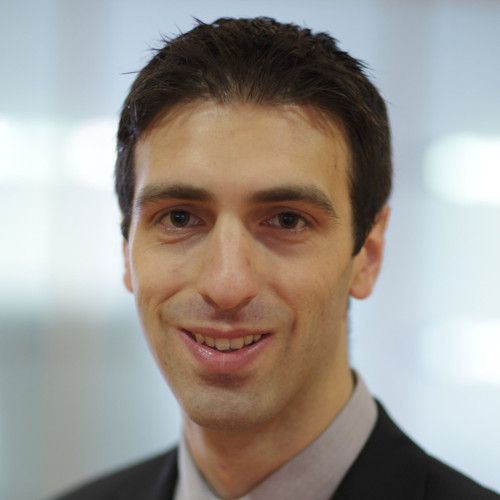
\includegraphics[height=2.0cm]{images/michael-aeberhard-profile.jpg} \\
    \end{column}
\end{columns}
\end{frame}

\begin{frame}
\frametitle{About Me}
\framesubtitle{Career}
\begin{columns}[T]
    \begin{column}{.70\textwidth}
    \begin{itemize}
        \item BMW AG (2010-2018)
        \begin{itemize}
            \item Research in sensor data fusion
            \item Involved in German/EU funded reserach projects:
                SmartSenior, UR:BAN, AdaptIVe
            \item Developer, Product Owner, Project Lead for autonomous driving
        \end{itemize}
        \item Autonomus Intelligent Driving GmbH (2018-2020)
        \begin{itemize}
            \item Developer and Tech Lead for L4 "robot taxi" application
        \end{itemize}
        \item \href{https://www.apex.ai/}{Apex.AI} (2020-)
        \begin{itemize}
            \item Head of Application Engineering
            \item Bringing a safety-certified version ROS 2 to series production
        \end{itemize}
    \end{itemize}
    \end{column}
    \begin{column}{.30\textwidth}
    \centering
    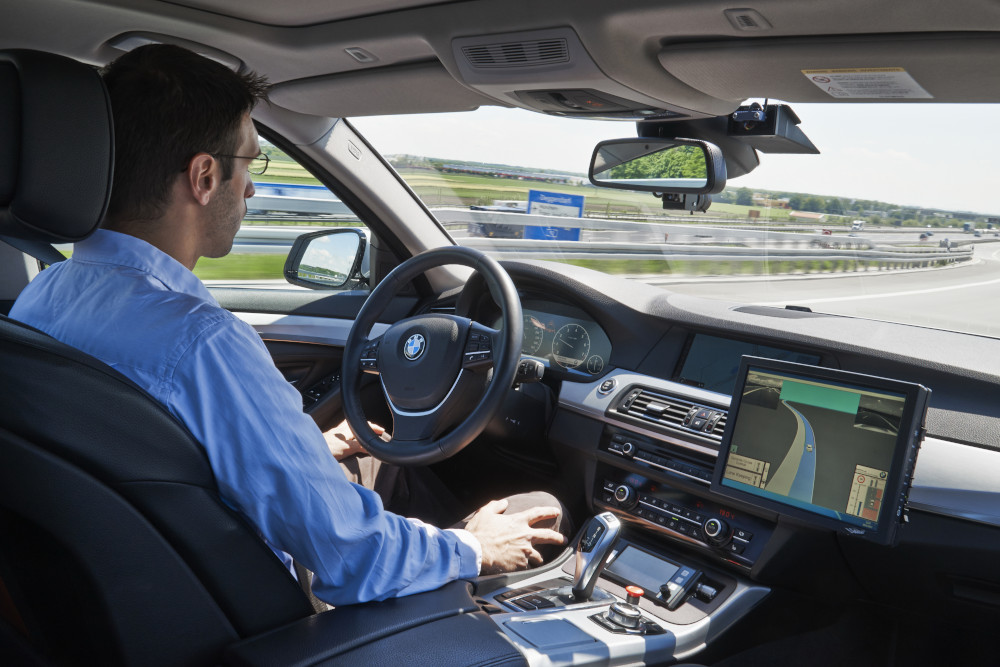
\includegraphics[height=2.0cm]{images/michael-aeberhard-bmw.jpg} \\
    \tiny \copyright \, 2013 BMW AG
    \end{column}
\end{columns}
\end{frame}
\begin{frame}
\frametitle{History of Autonomous Vehicles Development}
\framesubtitle{The Early Years (1990s)}
\begin{columns}[T]
    \begin{column}{.5\textwidth}
    \centering
    Prometheus Project \\
    \vspace{0.25cm}
    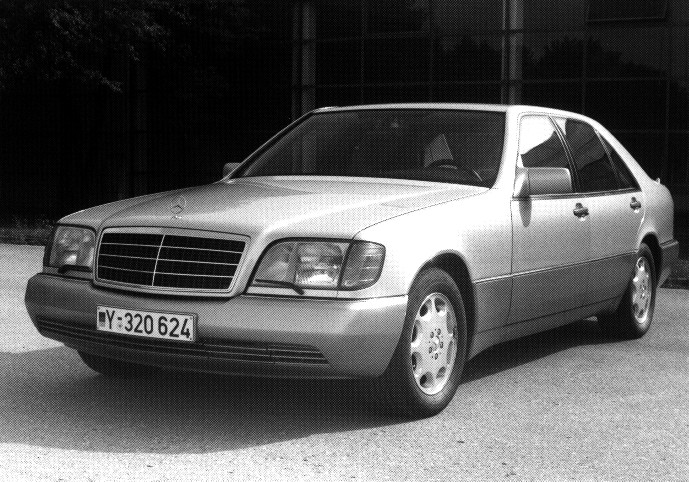
\includegraphics[height=2.2cm]{images/vamp.jpg} \\
    \tiny{\cite{Dickmanns1994} VaMP}
    \footnotesize
    \begin{itemize}
        \item European R\&D project (1985 - 1995)
        \item Prof. Ernst Dickmann's research vehicles
            demonstrated 1,000+ km automated highway drives
    \end{itemize}
    \end{column}
    \pause
    \begin{column}{.5\textwidth}
    \centering
    Demo '97 \\
    \vspace{0.25cm}
    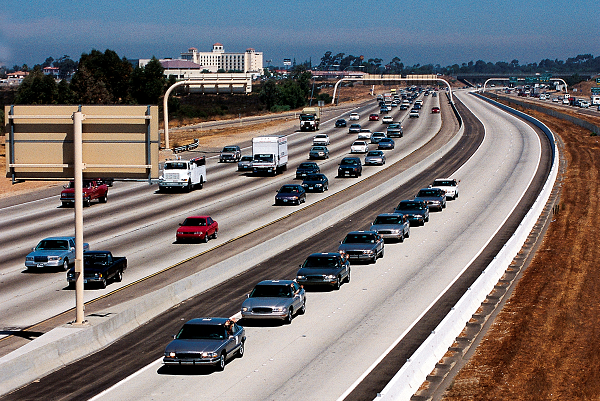
\includegraphics[height=2.2cm]{images/demo-97-no-hands.png} \\
    \tiny{Platoon demo}\footnotemark[1]
    \footnotesize
    \begin{itemize}
        \item US DOT sponsored research to demonstrate the
            Automated Highway System (AHS)
        \item A 12 km stretch of an HOV lane was used for the demonstration
    \end{itemize}
    \end{column}
\end{columns}
\pause
\footnotesize
\begin{block}{}
These projects set the foundation for OEM ADAS development in the
2000s
\end{block}
\footnotetext[1]{\tiny{\url{https://path.berkeley.edu/research/connected-and-automated-vehicles/national-automated-highway-systems-consortium}}}
\end{frame}

\begin{frame}
\frametitle{History of Autonomous Vehicles Development}
\framesubtitle{The DARPA Challenges (2004-2008)}
\begin{columns}[T]
    \begin{column}{.65\textwidth}
    DARPA Grand Challenges\footnotemark[1]
    \begin{itemize}
        \item In the 2004 competition, 15 teams competed for a \$1 million prize
            on a 240 km desert route
        \item The prize went unclaimed; the best team was able to complete
            11.78 km
        \item In 2005, a \$2 million prize was up for grabs on a 212 km route
        \item The team from Stanford University with their vehicle
            \emph{Stanley} completed the course the fastest (in total 5 teams
            completed the course)
    \end{itemize}
    \end{column}
    \begin{column}{.35\textwidth}
    \centering
    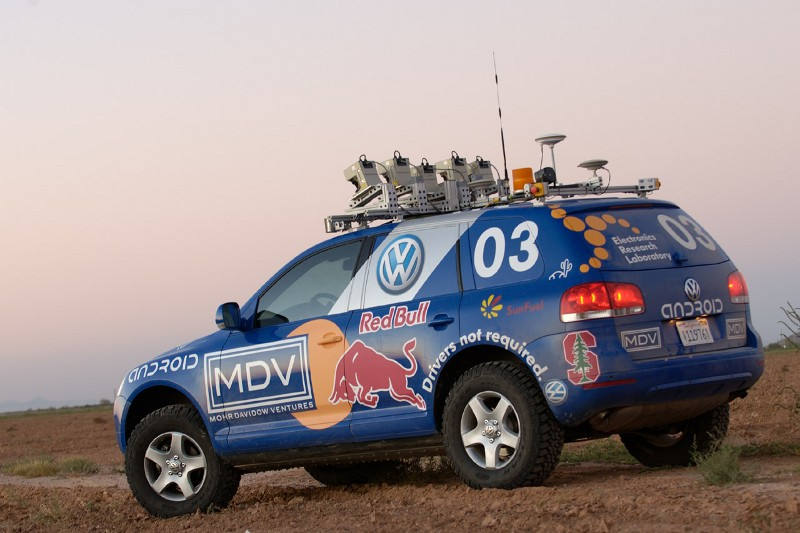
\includegraphics[height=3cm]{images/darpa_stanley.jpg} \\
    \tiny{\cite{DARPAStanley}}
    \end{column}
\end{columns}
\footnotetext[1]{\tiny{\url{https://www.darpa.mil/about-us/timeline/-grand-challenge-for-autonomous-vehicles}}}
\end{frame}
    
\begin{frame}
\frametitle{History of Autonomous Vehicles Development}
\framesubtitle{The DARPA Challenges (2004-2008)}
\begin{columns}[T]
    \begin{column}{.6\textwidth}
    DARPA Urban Challenge\footnotemark[1]
    \begin{itemize}
        \item In 2007, a third competition for a \$2 million prize was held on
            a 96 km urban route
        \item A total of 11 teams competed in the final competition
        \item A team from Carnegie Melon University won with their vehicle
            \emph{Boss}
    \end{itemize}
    \end{column}
    \begin{column}{.4\textwidth}
    \centering
    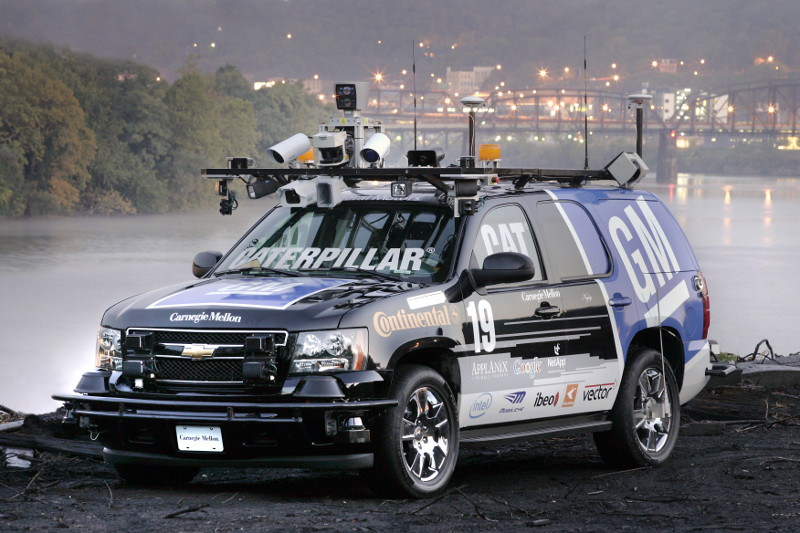
\includegraphics[height=3cm]{images/darpa_boss.jpg} \\
    \tiny{\cite{CMUUrbanChallenge}}
    \end{column}
\end{columns}
\pause
\vspace{0.25cm}
\begin{block}{}
The student, engineers, and companies of the DARPA challenges laid the
foundations for today's autonomous driving development and are leaders in the
industry.
\end{block}
\footnotetext[1]{\tiny{\url{https://www.darpa.mil/about-us/timeline/darpa-urban-challenge}}}
\end{frame}

\begin{frame}
\frametitle{History of Autonomous Vehicles Development}
\framesubtitle{The Industry Ramp-Up Phase (2010-2020)}
\centering OEMs and Tier 1s
\begin{columns}[T]
    \begin{column}{.25\textwidth}
        \centering
        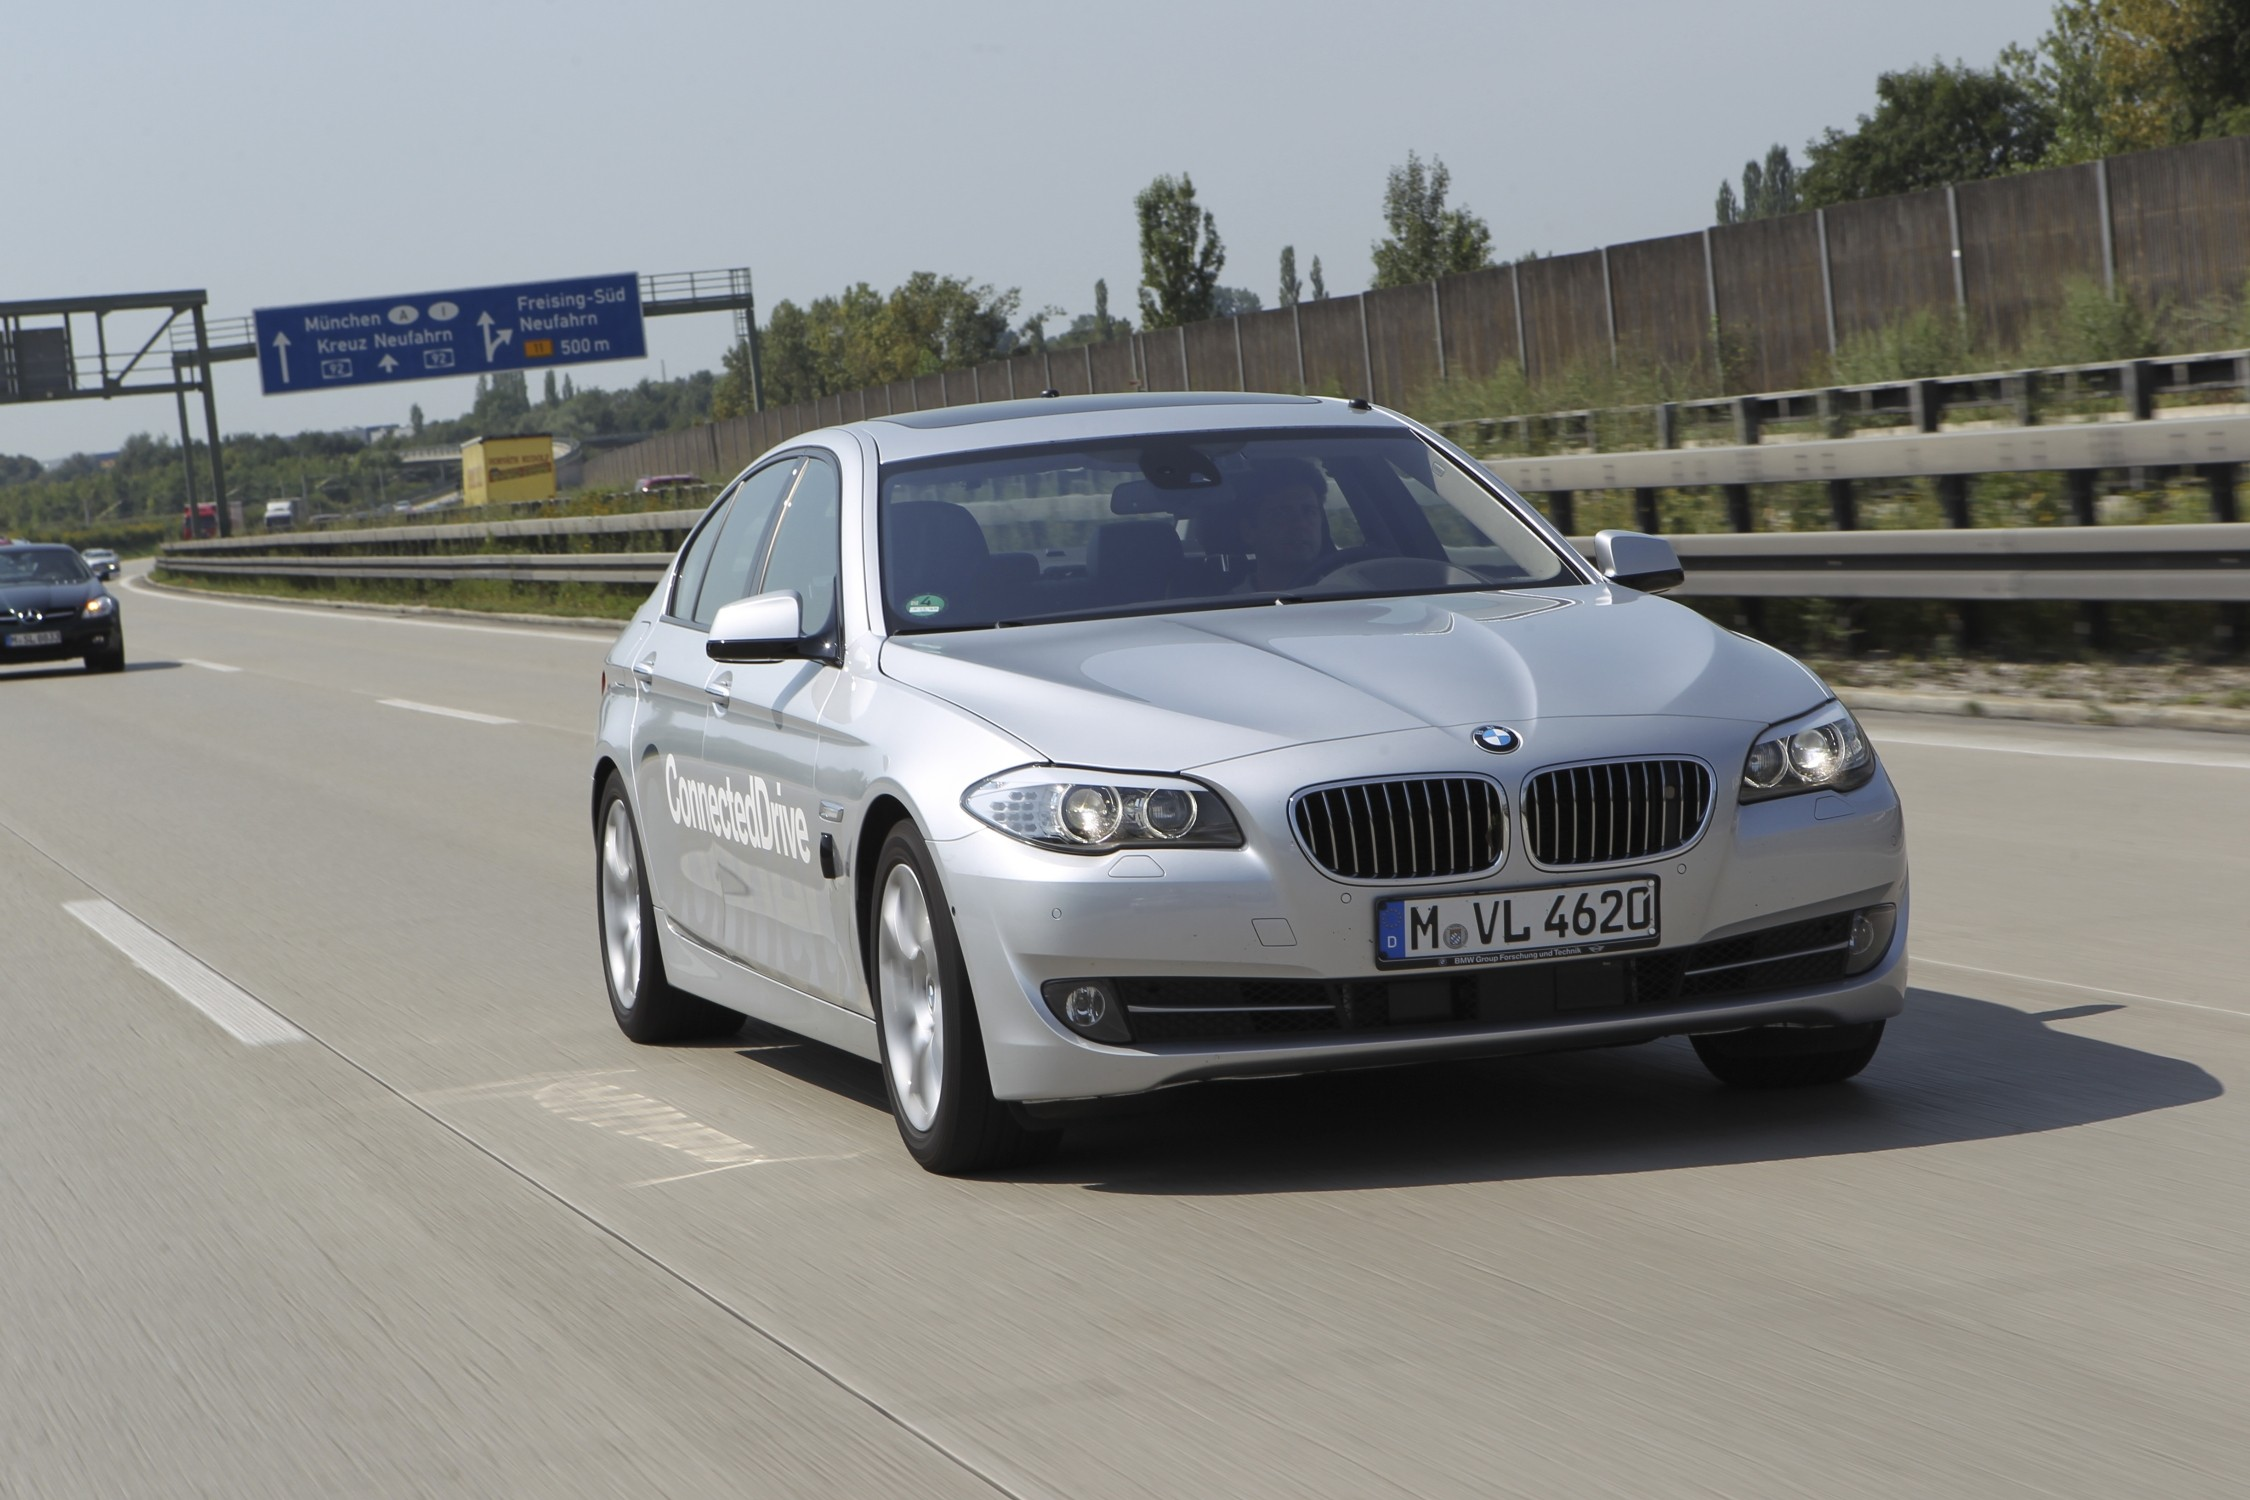
\includegraphics[height=1.9cm]{images/bmw_had.jpg} \\
        \footnotesize BMW \cite{AeberhardBMWHAF2015}
    \end{column}
    \begin{column}{.25\textwidth}
        \centering
        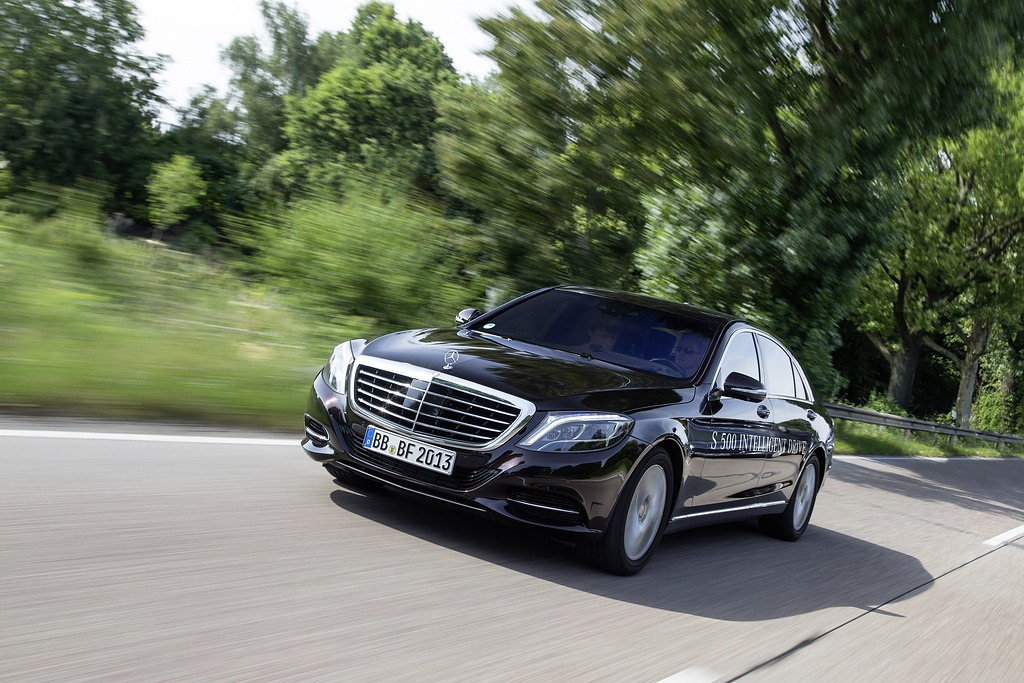
\includegraphics[height=1.9cm]{images/mercedes_bertha_benz_drive.jpg} \\
        \footnotesize Mercedes-Benz \cite{DaimlerBertha2014}
    \end{column}
    \begin{column}{.25\textwidth}
        \centering
        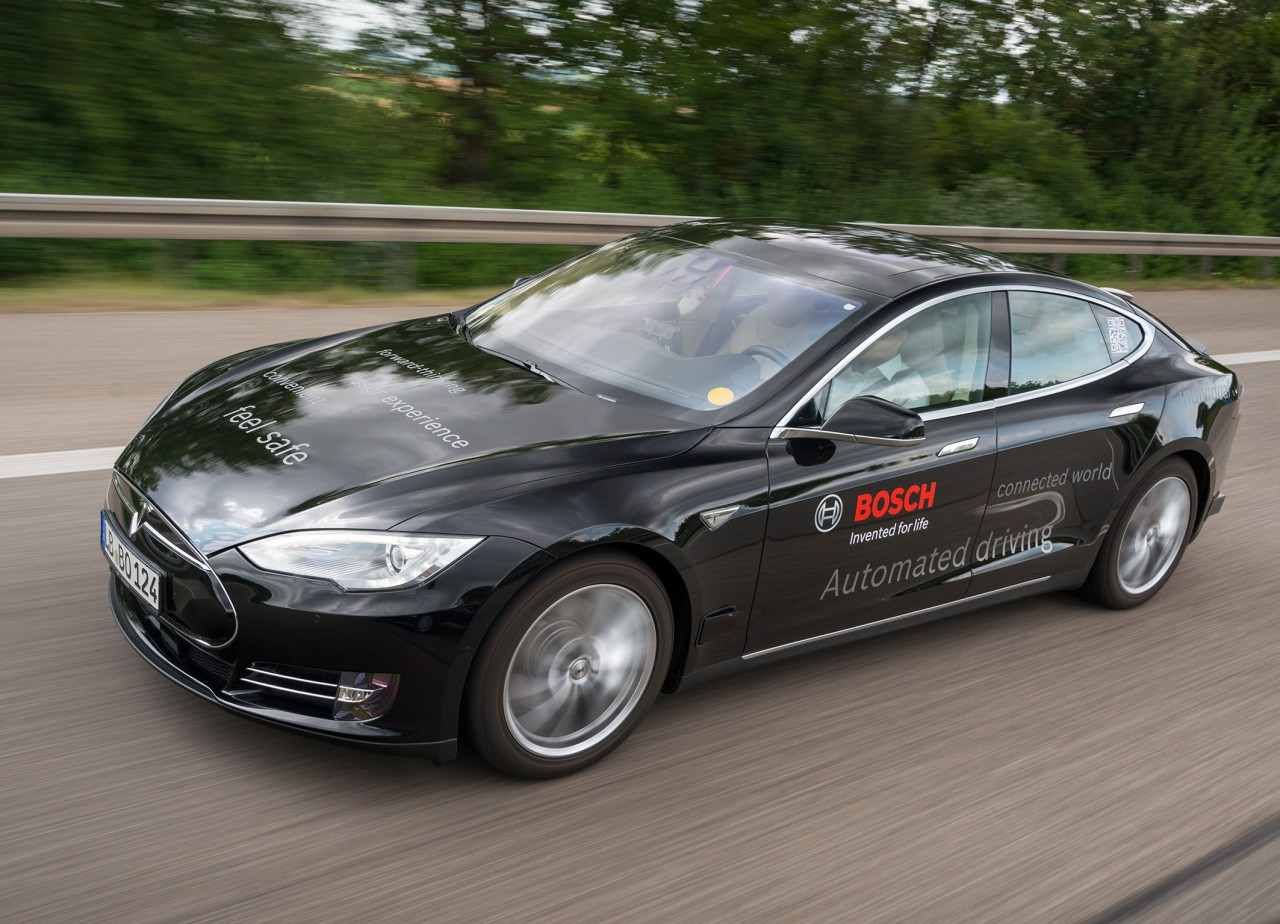
\includegraphics[height=1.9cm]{images/bosch_had.jpg} \\
        \footnotesize Bosch \cite{BoschPressHAD}
    \end{column}
    \begin{column}{.25\textwidth}
        \centering
        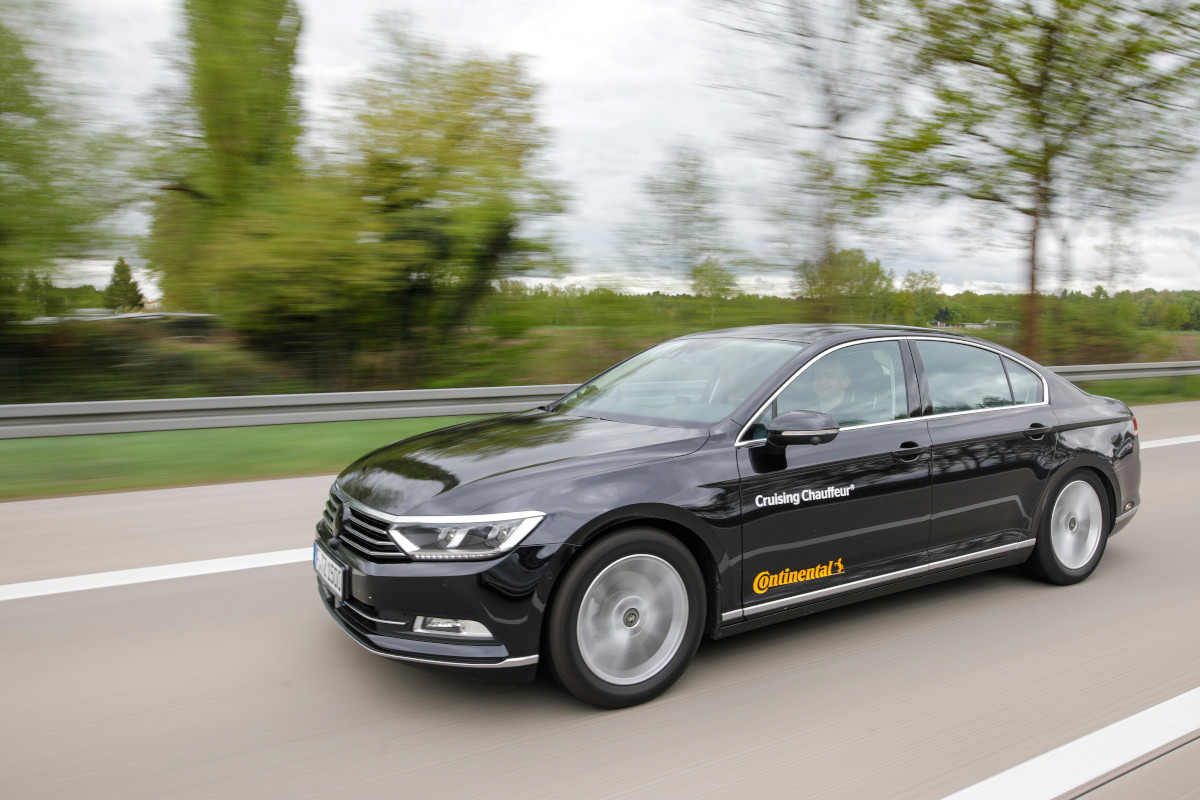
\includegraphics[height=1.9cm]{images/continental_had.jpg} \\
        \footnotesize Continental \cite{ContinentalHAD}
    \end{column}
\end{columns}
\vspace{0.5cm}
\centering New Players
\begin{columns}[T]
    \begin{column}{.25\textwidth}
        \centering
        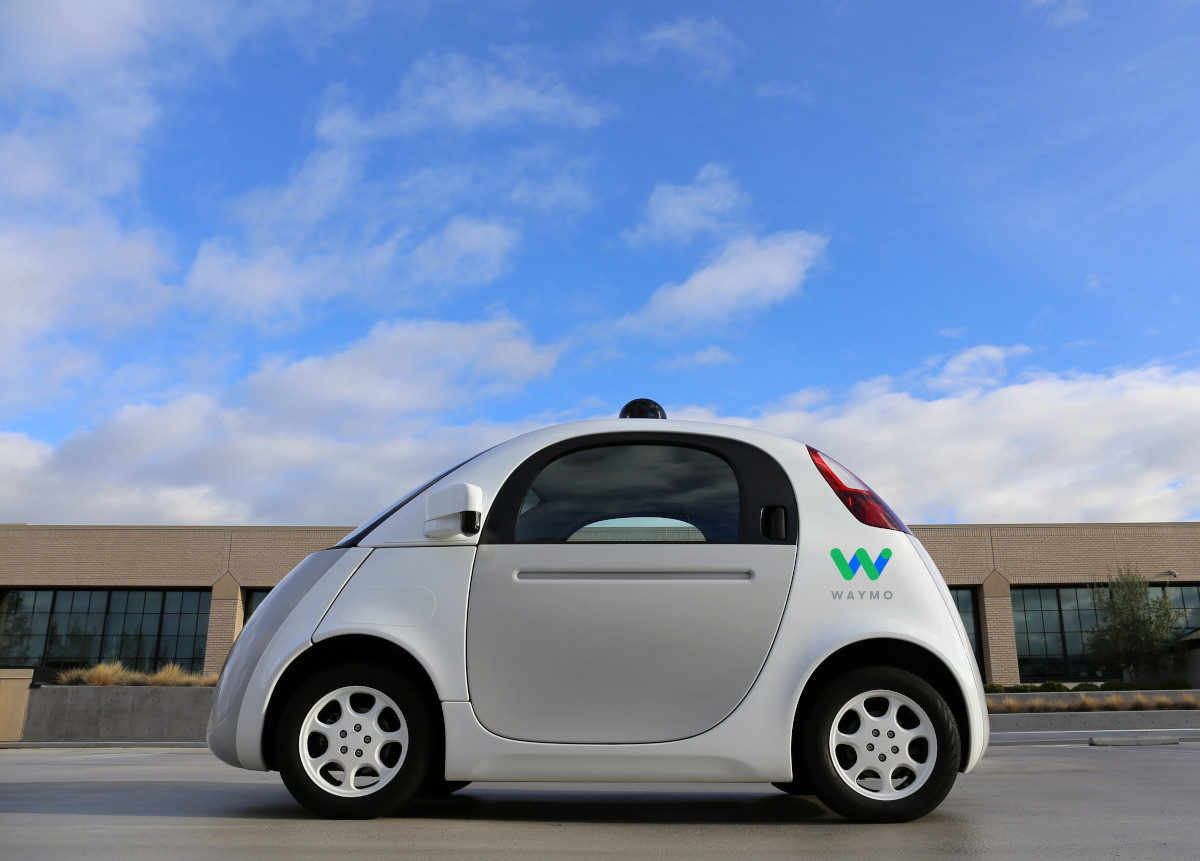
\includegraphics[height=1.9cm]{images/waymo_firefly.jpg} \\
        \footnotesize Waymo \cite{WaymoPress}
    \end{column}
    \begin{column}{.25\textwidth}
        \centering
        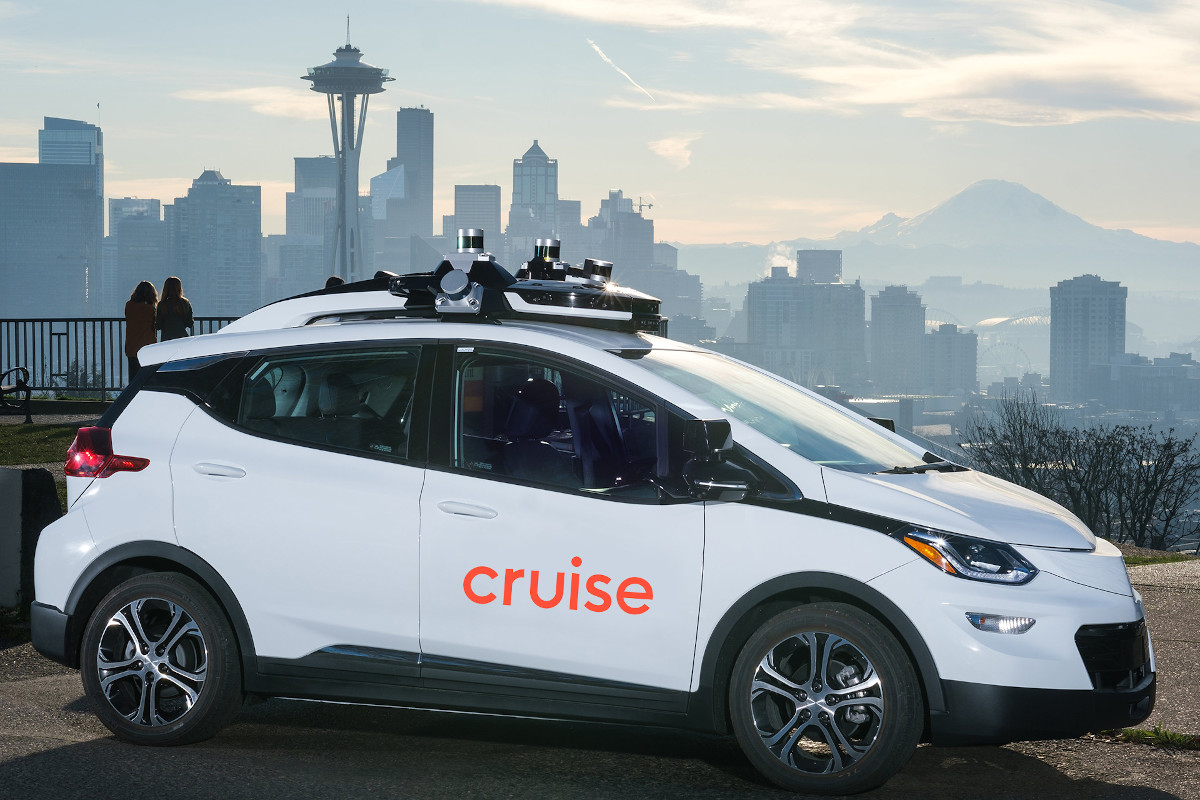
\includegraphics[height=1.9cm]{images/cruise_vehicle.jpg} \\
        \footnotesize Cruise \cite{CruiseNews}
    \end{column}
    \begin{column}{.25\textwidth}
        \centering
        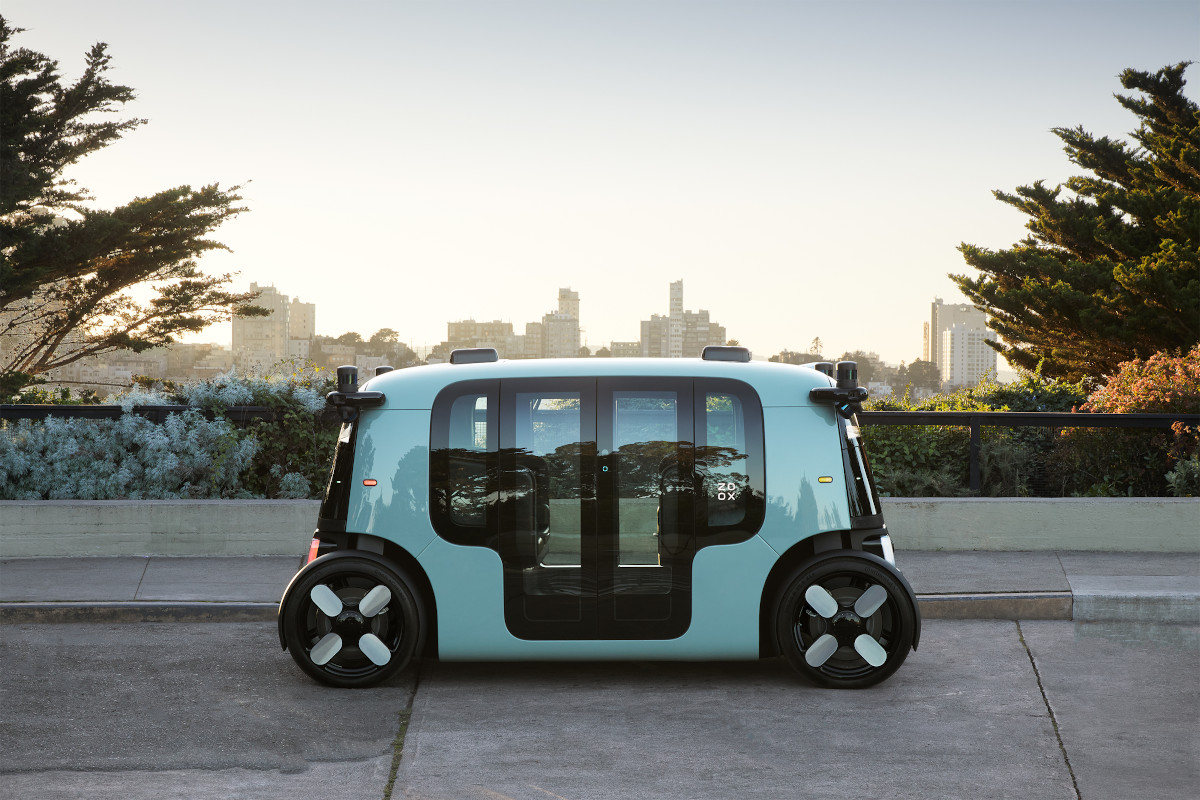
\includegraphics[height=1.9cm]{images/zoox_vehicle.jpg} \\
        \footnotesize Zoox \cite{ZooxPress}
    \end{column}
    \begin{column}{.25\textwidth}
        \centering
        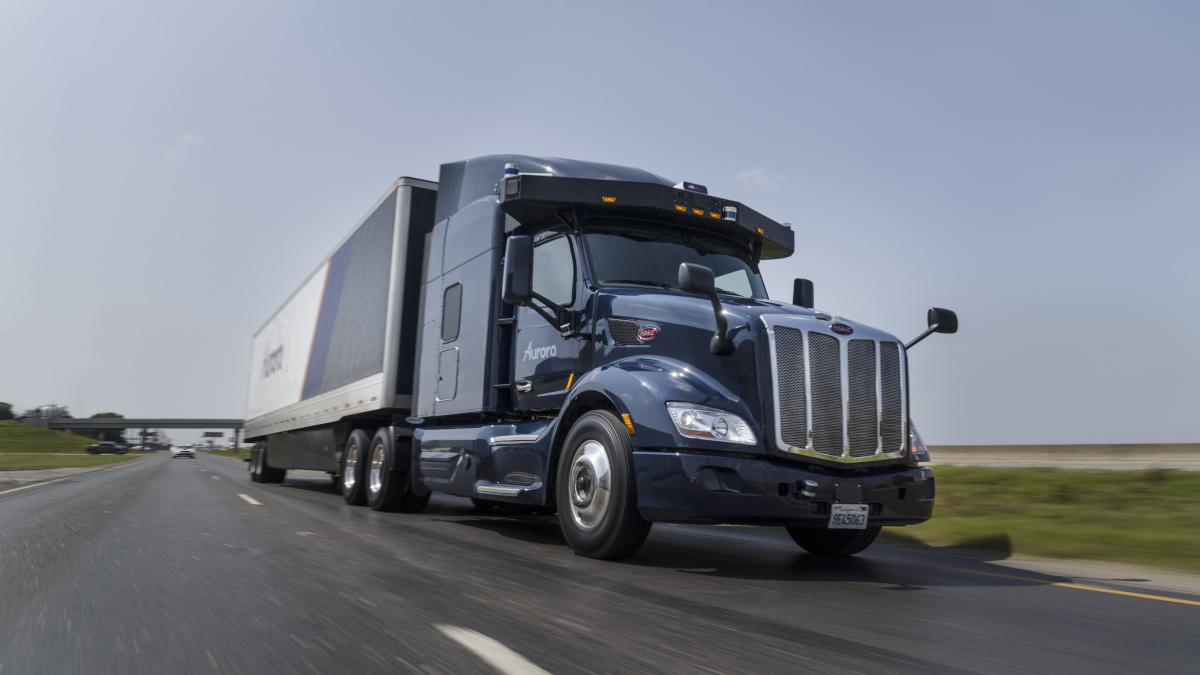
\includegraphics[height=1.9cm]{images/aurora_truck.jpg} \\
        \footnotesize Aurora \cite{AuroraMedia}
    \end{column}
\end{columns}
\end{frame}

\begin{frame}
\frametitle{History of Autonomous Vehicles Development}
\framesubtitle{Going to Production (2020 - ???)}
Only since 2020 have the first true driveless vehicles been allowed to operate
on public roads, albeit in limited numbers and locations.\\
\begin{columns}[]
    \begin{column}{0.33\textwidth}
        \centering
        \includegraphics[height=2.5cm]{images/waymo_one.jpg} \\
        \footnotesize Waymo One\footnotemark[1]
    \end{column}
    \begin{column}{0.33\textwidth}
        \centering
        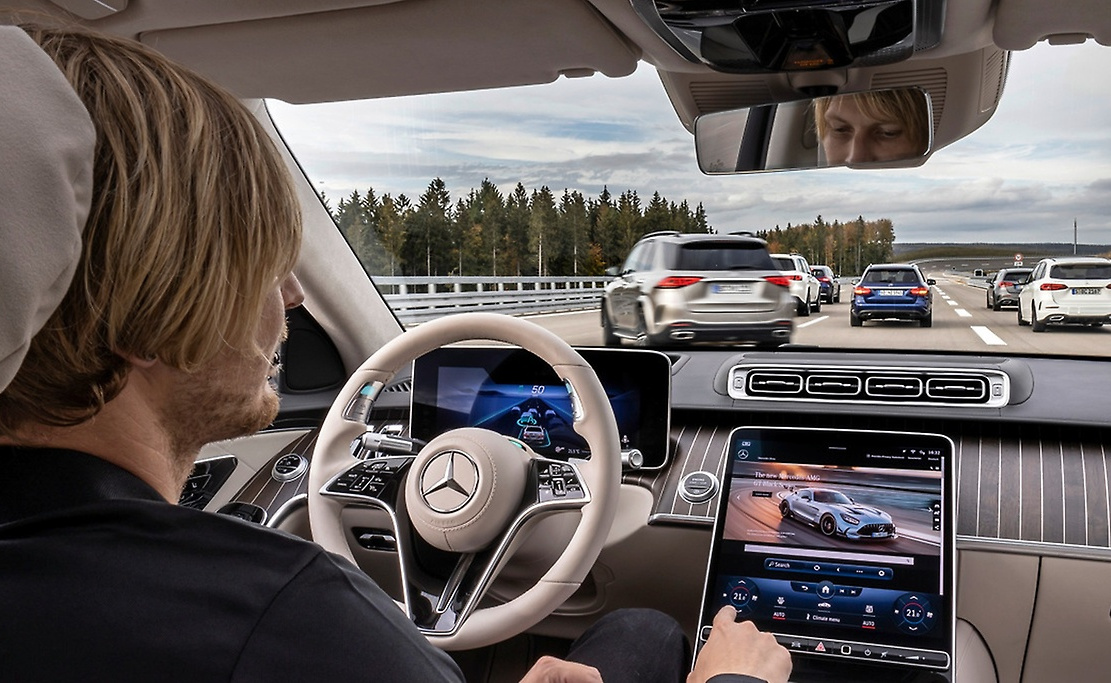
\includegraphics[height=2.5cm]{images/mercedes-level-3.jpg} \\
        \footnotesize Mercedes-Benz DRIVE PILOT \cite{MercedesLevel3}
    \end{column}
    \begin{column}{0.33\textwidth}
        \centering
        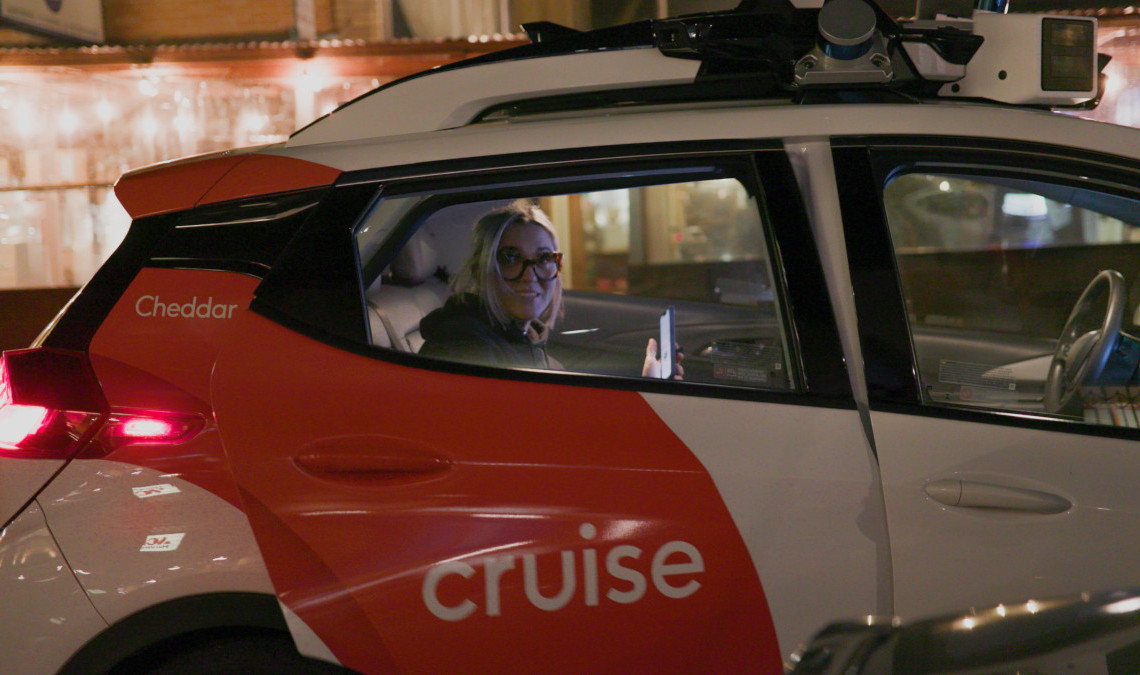
\includegraphics[height=2.5cm]{images/cruise_riders.jpg} \\
        \footnotesize Cruise Riders \footnotemark[2]
    \end{column}
\end{columns}
\begin{block}{}
The next decade will be the beginning of the commercialization of autonomous
vehicles. Many challenges remain for widespread adoption...
\end{block}
\footnotetext[1]{\tiny{\url{https://waymo.com/waymo-one/}}}
\footnotetext[2]{\tiny{\url{https://getcruise.com/rides/}}}
\end{frame}

% SDV, Vehicle OS --> slide about trends (McKinsey report?)

\begin{frame}
\frametitle{The Software Challenge}
Modern vehicles are smartphones on wheels and the next generation vehicles
will automated the driving task.\\
$\Rightarrow$ Software is taking over the automotive industry
\vspace{0.25cm}
\begin{itemize}
    \item Dozens of ECUs in a modern vehicle
    \item High-resolution displays for the drive and passenger
    \item Sensors detect the vehicle's environment
    \item Actuators automatically control many vehicle functions
    \item Thousands of software developers from many companies collaborating
    \item Safety of utmost importance
\end{itemize}
\end{frame}

\begin{frame}
\frametitle{The Software Challenge}
\framesubtitle{Autonomous Driving}
For an autonomous vehicle system, a very high-dimensional input space from
environment sensing sensors and vehicle sensors must be translated,
\textbf{with software}, into steering, brake and motor controls.\\
\begin{block}{}
Creating an autonomous driving system is an incredibly complex task that even
challenges humans.
\end{block}
\end{frame}

\begin{frame}
\frametitle{The Phases of Development}
Autonomous vehicles and ADAS development has traditionally followed three phases
of development.

\begin{itemize}
    \item \textbf{Research}: Develop prototypes to understand the use-cases, algorithms,
        hardware, etc. $\rightarrow$ is the product feasible?
    \item \textbf{Pre-development}: Iron out the details, requirements, commercial
        viability, etc. $\rightarrow$ develop a solid blue print for production
    \item \textbf{Production}: Software and hardware is hardened and optimized for
        production quality and cost, meeting any required safety, automotive or
        product standards
\end{itemize}
\pause
\begin{block}{}
The autonomous driving industry today is making the transition from
pre-development to production.
\end{block}
\end{frame}

\begin{frame}
\frametitle{Architecture}
The architecture of a system can be broken down into different levels
of detail.
\begin{itemize}
    \item \textbf{Functional Architecture}: Logical components and sub-systems,
        along with a high-level definition of interfaces, are identified
    \item \textbf{Software Architecture}: Implementation of logical components
        into concrete software components with concrete interface
        implementations
    \item \textbf{Hardware Architecture}: Partitioning of the software
        components onto specific hardware and defining the low-level
        communication mechanisms of the components
\end{itemize}
The different phases of development will focus on different levels of
the architecture and hence specific details of the system.
\end{frame}

\section{Functional Architecture}

\subsection{Introduction}

\begin{frame}
\frametitle{Functional Architecture}
The functional architecture is initially developed during the research phase
and refined as development matures to production.

\begin{itemize}
    \item The main components of a system are identified
    \item Specific algorithms which realize the components are developed
    \item High-level interfaces between components are created
\end{itemize}

\begin{block}{}
The functional architecture for an autonomous driving vehicle has evolved
over the past decade and is converging towards an industry standard.
\end{block}
\end{frame}

\begin{frame}
\frametitle{Sense - Plan - Act}
\framesubtitle{Common Autonomous Vehicle Functional Architecture}
The \emph{Sense - Plan - Act} architecture is still predominant in modern autonomous
vehicle architectures.

\vspace{1cm}

\begin{center}
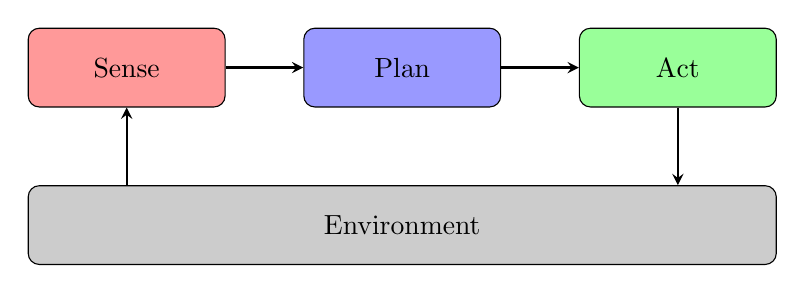
\begin{tikzpicture}[node distance=3.5cm]
    \node (sense)[rectangle,rounded corners,minimum width=2.5cm,minimum height=1cm,text centered,draw=black,fill=red!40]{Sense};
    \node (plan)[right of=sense,rectangle,rounded corners,minimum width=2.5cm,minimum height=1cm,text centered,draw=black,fill=blue!40]{Plan};
    \node (act)[right of=plan,rectangle,rounded corners,minimum width=2.5cm,minimum height=1cm,text centered,draw=black,fill=green!40]{Act};
    \node (environment)[below of=plan,yshift=1.5cm,rectangle,rounded corners,minimum width=9.5cm,minimum height=1cm,text centered,draw=black,fill=gray!40]{Environment};
    \draw [thick,->,>=stealth] (sense) -- (plan);
    \draw [thick,->,>=stealth] (plan) -- (act);
    \draw [thick,->,>=stealth] (act) -- ([xshift=3.5cm]environment.north);
    \draw [thick,<-,>=stealth] (sense) -- ([xshift=-3.5cm]environment.north);
    \end{tikzpicture}
\end{center}
\end{frame}

\begin{frame}
\frametitle{Sense - Plan - Act}
\framesubtitle{Common Autonomous Vehicle Functional Architecture}
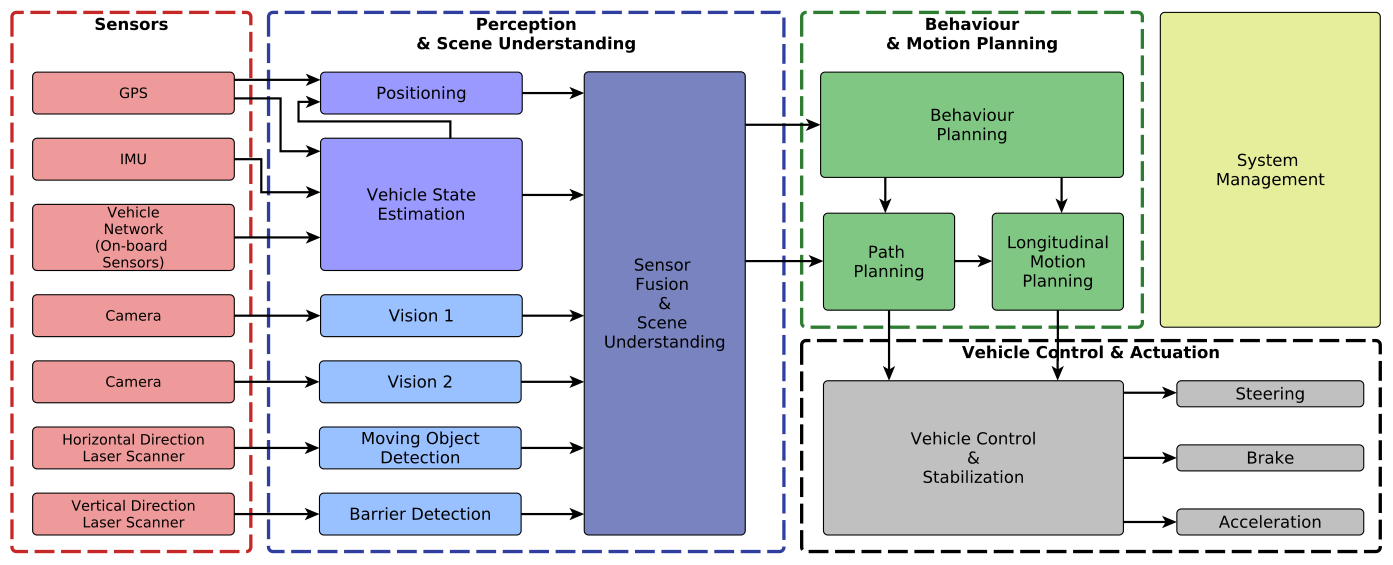
\includegraphics[width=\textwidth]{images/tas_2016_fig4_av_functional_architecture.png}
\tiny{Architecture image from \cite{Tas2016-sd} based on the vehicle that won the
Korean Autonomous Vehicle Competition \cite{Jo2014-na}}.
\end{frame}

\subsection{Sensors}

\begin{frame}
\frametitle{Sensors}
Autonomous vehicles use a combination of cameras, radar and lidar sensors to
sense and perceive the environment. \\
\vspace{0.25cm}
\centering
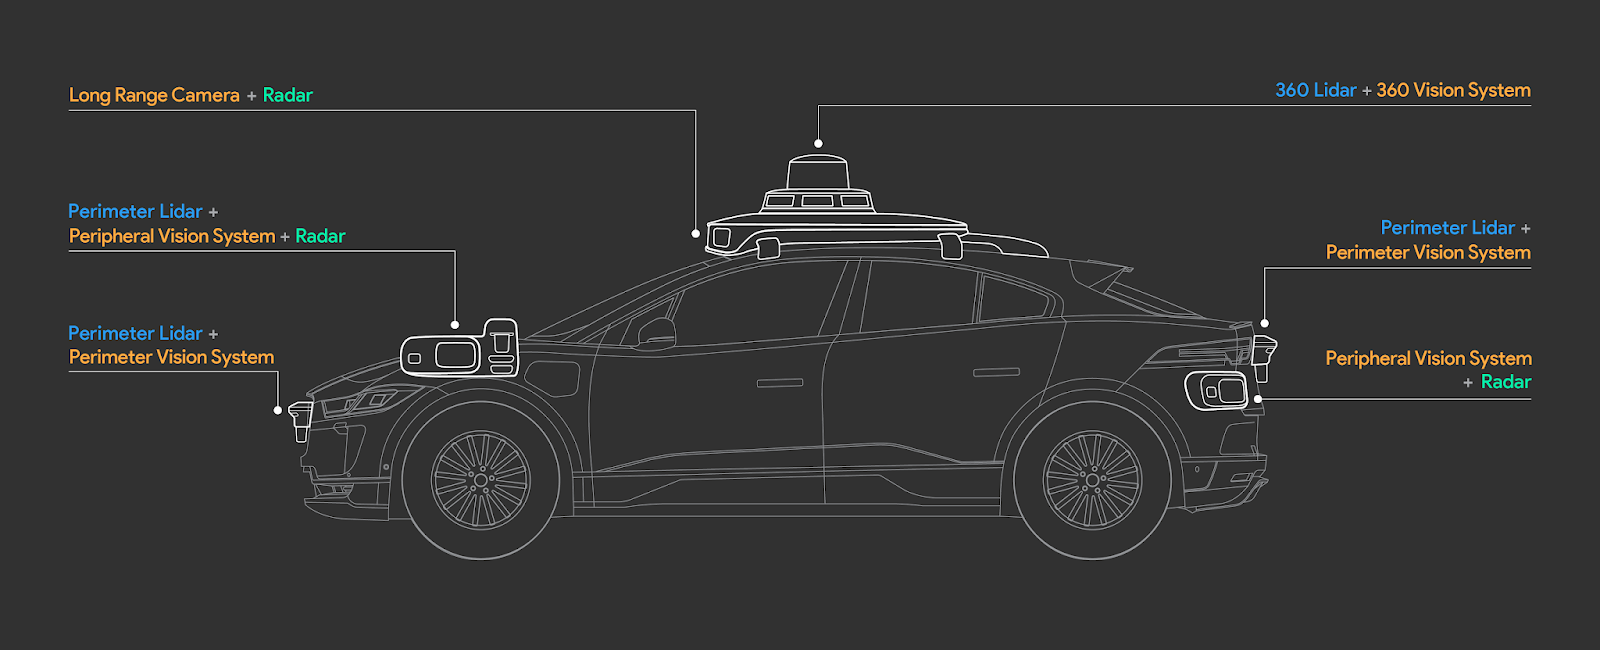
\includegraphics[width=0.9\textwidth]{images/waymo_sensors.png}\\
\footnotesize{Waymo sensor suite\footnotemark[1]}
\footnotetext[1]{\tiny{\url{https://blog.waymo.com/2020/03/introducing-5th-generation-waymo-driver.html}}}
\end{frame}

\begin{frame}
\frametitle{Sensors}
\framesubtitle{Camera}
\begin{columns}[T]
    \begin{column}{.5\textwidth}
        \centering
        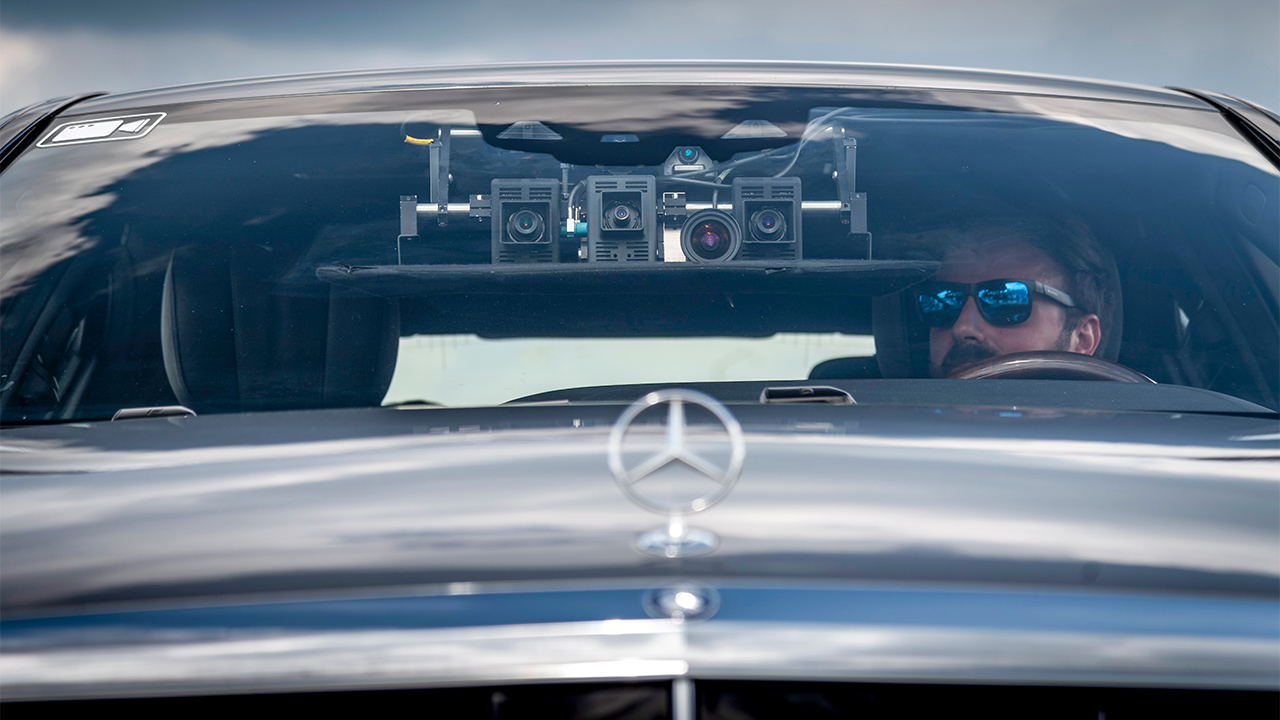
\includegraphics[width=0.6\textwidth]{images/daimler_cameras.jpg}\\
        \tiny{Source: Daimler\footnotemark[1]}\\
        \vspace{0.3cm}
        \href{https://www.youtube.com/watch?v=rACZACXgreQ}{
        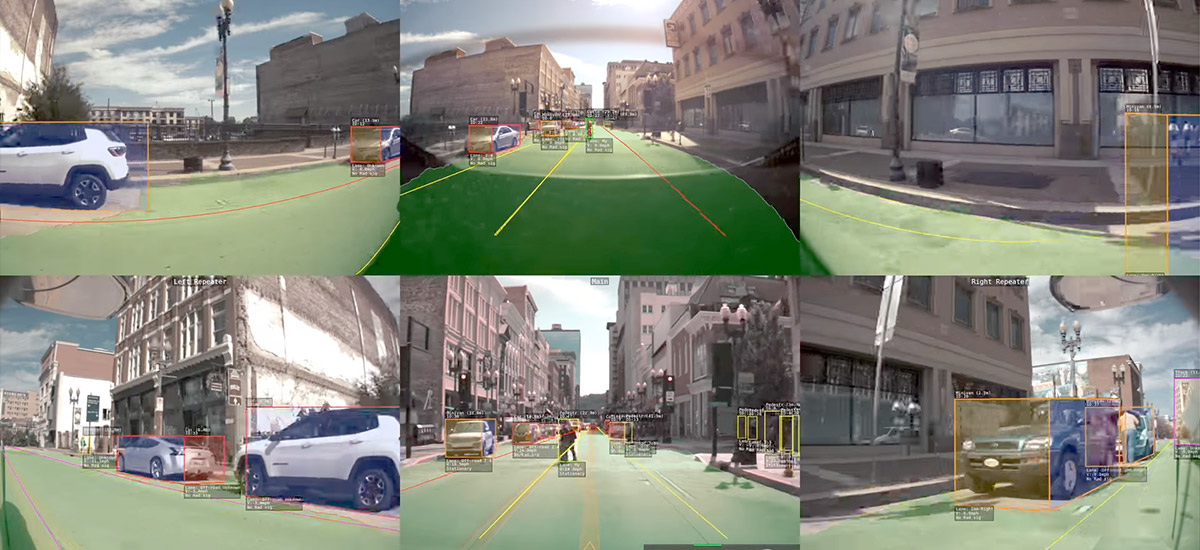
\includegraphics[width=0.9\textwidth]{images/tesla_autopilot_cameras.jpg}}\\
        \tiny{Tesla camera system, Source: YouTube (greentheonly)\footnotemark[2]}
    \end{column}
    \begin{column}{.5\textwidth}
        \footnotesize
        Vision sensors are the basis for an autonomous driving system, providing
        important perception input for many different purposes.
        \vspace{0.25cm}
        \begin{columns}[T]
            \begin{column}{0.45\textwidth}
                \footnotesize
                Capabilities:
                \begin{itemize}
                    \item Dynamic object detection
                    \item Static object detection
                    \item Lane and road detection
                    \item Classification
                    \item Traffic sign/light detection
                \end{itemize}
            \end{column}
            \begin{column}{0.55\textwidth}
                \footnotesize
                Important properties:
                \begin{itemize}
                    \item High dynamic range
                    \item $360\deg$ field of view
                    \item Global shutter
                    \item Low cost
                    \item No distance or velocity measurements
                \end{itemize}
            \end{column}
        \end{columns}
    \end{column}
\end{columns}

\footnotetext[1]{\tiny{\url{https://www.daimler.com/magazine/technology-innovation/automation-daimler-immendingen-camera-radar-lidar.html}}}
\footnotetext[2]{\tiny{\url{https://www.youtube.com/watch?v=rACZACXgreQ}}}
\end{frame}

\begin{frame}
\frametitle{Sensors}
\framesubtitle{Radar}
\begin{columns}[T]
    \begin{column}{.4\textwidth}
        \centering
        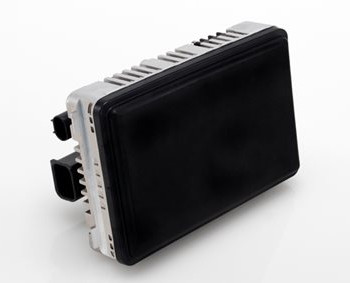
\includegraphics[width=0.3\textwidth]{images/continental_radar.jpg}\\
        \vspace{0.1cm}
        \tiny{Source: Continental\footnotemark[1]}\\
        \vspace{0.3cm}
        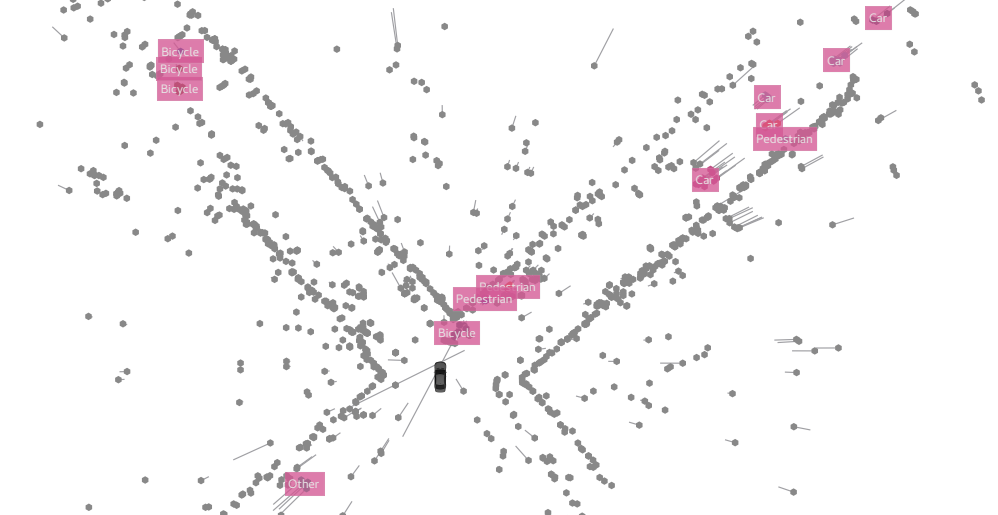
\includegraphics[width=\textwidth]{images/daimler_radar_dataset.png}\\
        \tiny{Source: Daimler, RadarScenes dataset\footnotemark[2]}
    \end{column}
    \begin{column}{.6\textwidth}
        \footnotesize
        Radar has been the workhorse of ADAS for over two decades, being the main
        sensor for ACC and continues its importance in autonomous driving systems.
        \vspace{0.2cm}
        \begin{columns}[T]
            \begin{column}{0.4\textwidth}
                \footnotesize
                Capabilities:
                \begin{itemize}
                    \item Dynamic object detection
                    \item Static object detection
                    \item Road boundary detection
                \end{itemize}
            \end{column}
            \begin{column}{0.6\textwidth}
                \footnotesize
                Important properties:
                \begin{itemize}
                    \item Robust in weather, e.g. rain, fog, etc.
                    \item Direct measurement of speed
                    \item Reasonable cost
                    \item Low resolution, poor vertical separation
                \end{itemize}
            \end{column}
        \end{columns}
    \end{column}
\end{columns}
\footnotetext[1]{\tiny{\url{https://www.continental-automotive.com/en-gl/Passenger-Cars/Autonomous-Mobility/Enablers/Radars/Long-Range-Radar/ARS540}}}
\footnotetext[2]{\tiny{\url{https://radar-scenes.com/}}}
\end{frame}

\begin{frame}
\frametitle{Sensors}
\framesubtitle{Lidar}
\begin{columns}[T]
    \begin{column}{.5\textwidth}
        \centering
        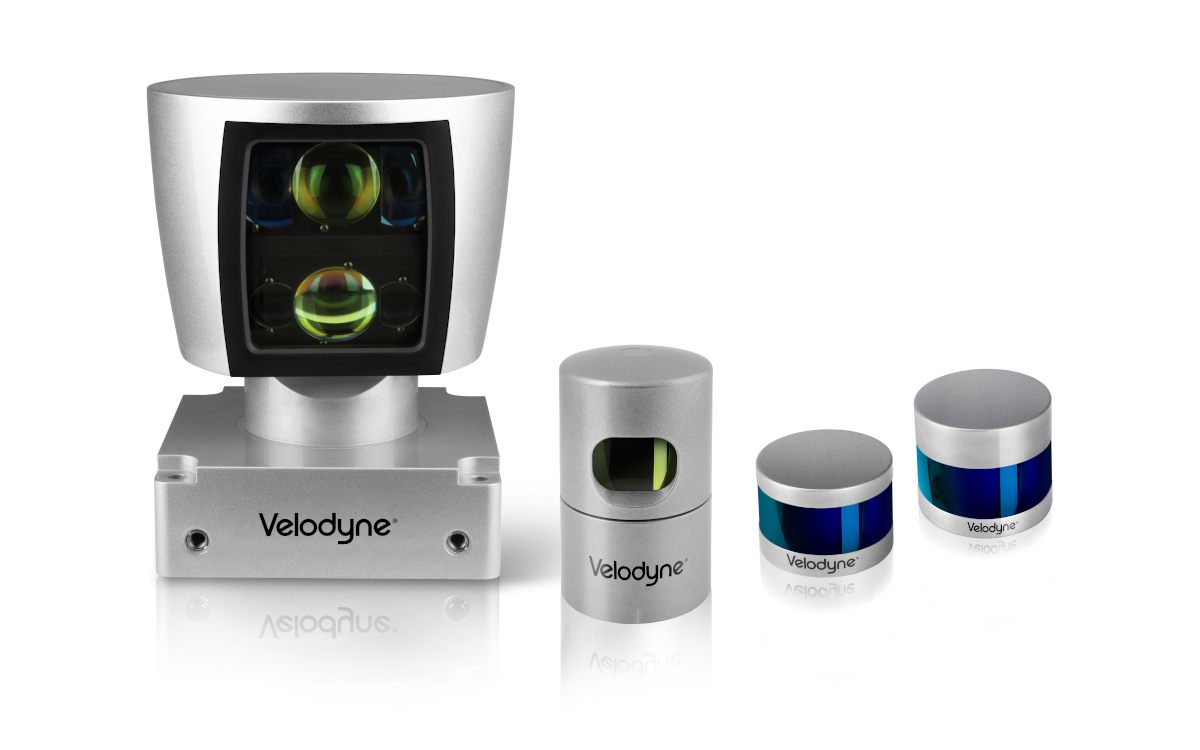
\includegraphics[width=0.5\textwidth]{images/velodyne_lidars.png}\\
        \vspace{0.2cm}
        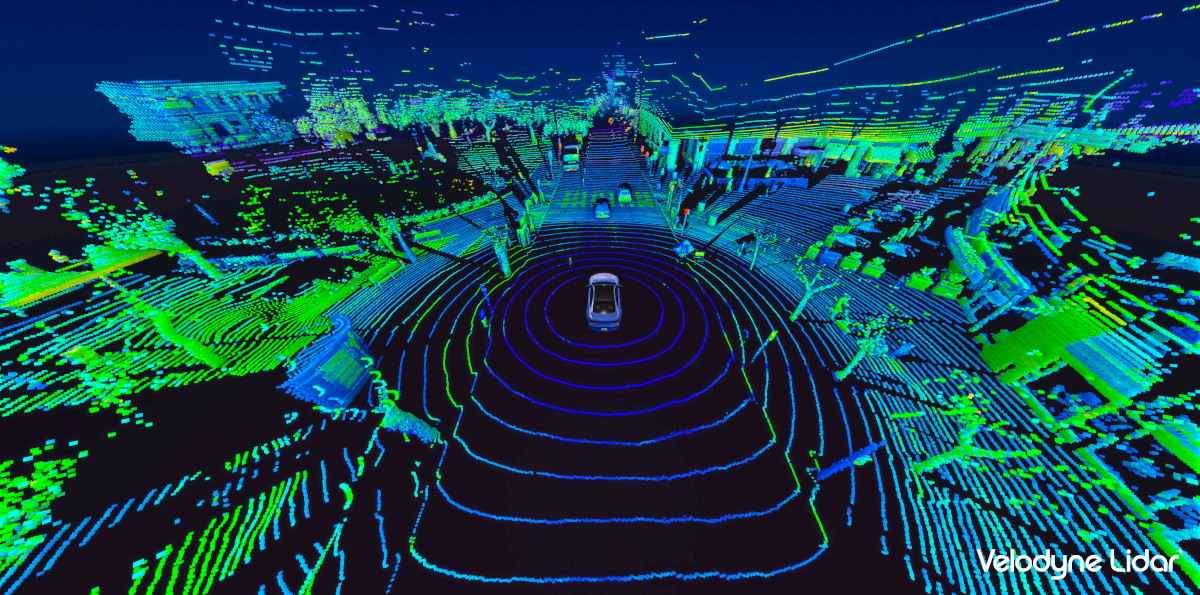
\includegraphics[width=\textwidth]{images/velodyne_pointcloud.jpg}\\
        \tiny{Source: Velodyne\footnotemark[1]}
    \end{column}
    \begin{column}{.5\textwidth}
        \footnotesize
        Only very recently has lidar been introduced in production vehicles, but it has
        been a core sensor of autonomous driving research since the DARPA challenges.
        \vspace{0.2cm}
        \begin{columns}[T]
            \begin{column}{0.4\textwidth}
                \footnotesize
                Capabilities:
                \begin{itemize}
                    \item Dynamic and static object detection
                    \item Road boundary and curb detection
                    \item Lane detection
                \end{itemize}
            \end{column}
            \begin{column}{0.6\textwidth}
                \footnotesize
                Important properties:
                \begin{itemize}
                    \item High resolution
                    \item Large field of view
                    \item Measure intensity
                    \item Poor weather robustness
                    \item No velocity measurement
                \end{itemize}
            \end{column}
        \end{columns}
    \end{column}
\end{columns}
\footnotetext[1]{\tiny{\url{https://velodynelidar.com/media-kit/}}}
\end{frame}

\subsection{Perception}

\begin{frame}
\frametitle{Perception}
\framesubtitle{Object Detection and Tracking}
\begin{columns}[T]
    \begin{column}{.45\textwidth}
        \centering
        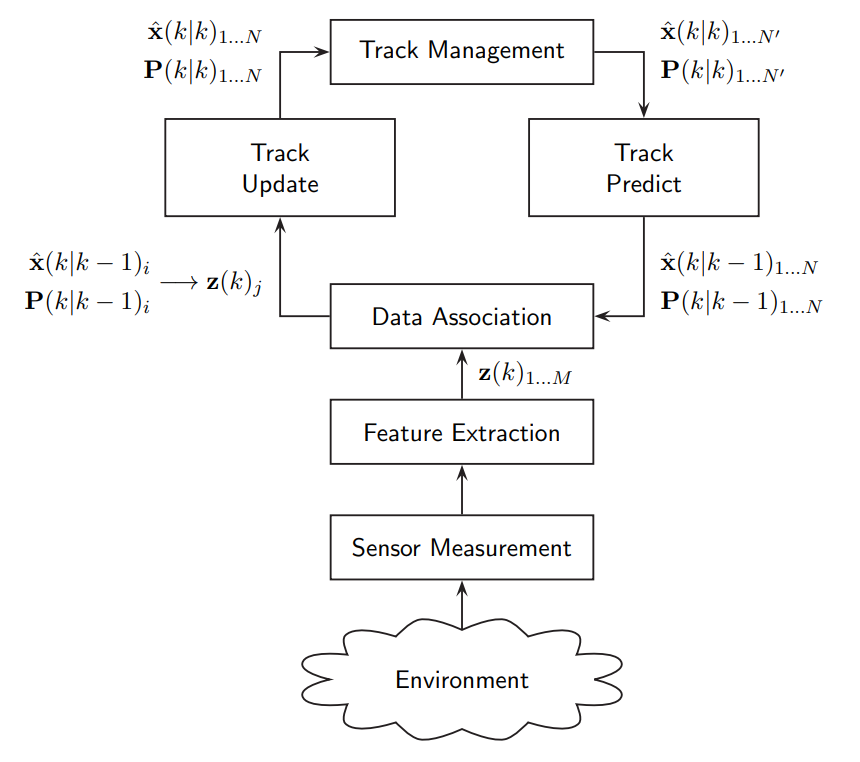
\includegraphics[width=0.75\textwidth]{images/aeberhard_tracking.png}\\
        \tiny{Common tracking architecture \cite{AeberhardDissertation}}\\
        \vspace{0.25cm}
        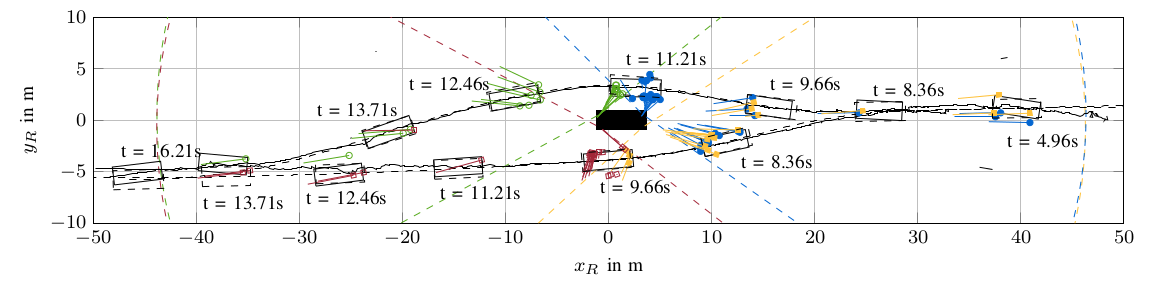
\includegraphics[width=\textwidth]{images/scheel_radar_tracking.png}\\
        \tiny{Tracking two objects with radar measurements \cite{Scheel2019}}
    \end{column}
    \begin{column}{.55\textwidth}
        Detection of dynamic objects is one of the central components in an
        AV system, with a very long history.
        \begin{itemize}
            \item Core algorithm is the Kalman filter \cite{Kalman1960}
                (and many variations therefore of) to estimate an object's
                state over time
            \item Bounding boxes are the most common representation form
            \item Pre-processing algorithms usually detect objects in a single
                data frame (clustering, ML-based detection, etc.)
        \end{itemize}
    \end{column}
\end{columns}
\end{frame}

\begin{frame}
\frametitle{Perception}
\framesubtitle{Occupancy Grids}
\begin{columns}[]
    \begin{column}{.5\textwidth}
        \centering
        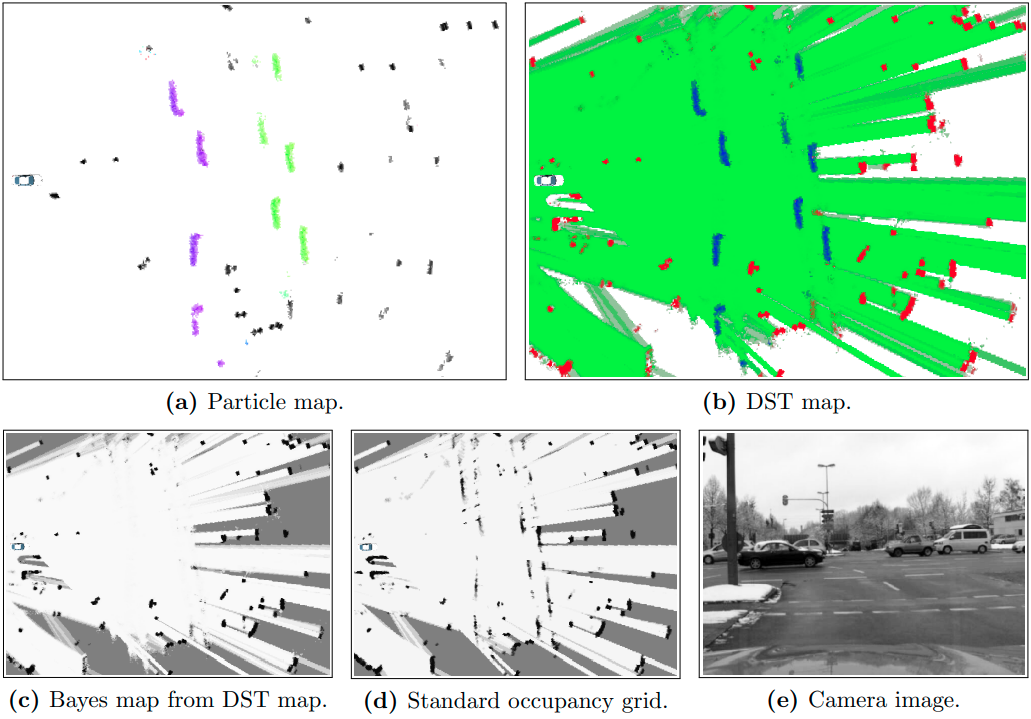
\includegraphics[width=\textwidth]{images/tanzmeister_dynamic_grids.png}\\
        \tiny{Dynamic occupancy grids \cite{TanzmeisterDissertation2016}}
    \end{column}
    \begin{column}{.5\textwidth}
        \footnotesize
        Occupancy grids have been a core algorithm in robotics since the
        mid-80s \cite{Moravec1985-ef} and have advanced ever since.
        \begin{itemize}
            \item Environment is rasterized into cells and a probability of
                occupancy is calculated
            \item Modern versions also calculate if a cell is dynamic or static
                or even the class (semantic)
            \item Free space (cells with no occupancy)
            \item Can be extended to include height information (elevation maps)
            \item Base environment representation which can be used by downstream
                component, e.g. object detection/tracking, localization, free space
                detection, etc.
        \end{itemize}
    \end{column}
\end{columns}
\end{frame}

\begin{frame}
\frametitle{Perception}
\framesubtitle{Lane / Road Detection}

\end{frame}

\begin{frame}
\frametitle{Perception}
\framesubtitle{Sensor Data Fusion}

\end{frame}

\subsection{Localization and Planning}

\begin{frame}
\frametitle{Localization}
Highly detailed maps for autonomous driving provide vital prior information
for navigating complex driving scenarios. Localization uses the sensor data
to localize the vehicle within such maps.\\
\vspace{0.25cm}
\centering
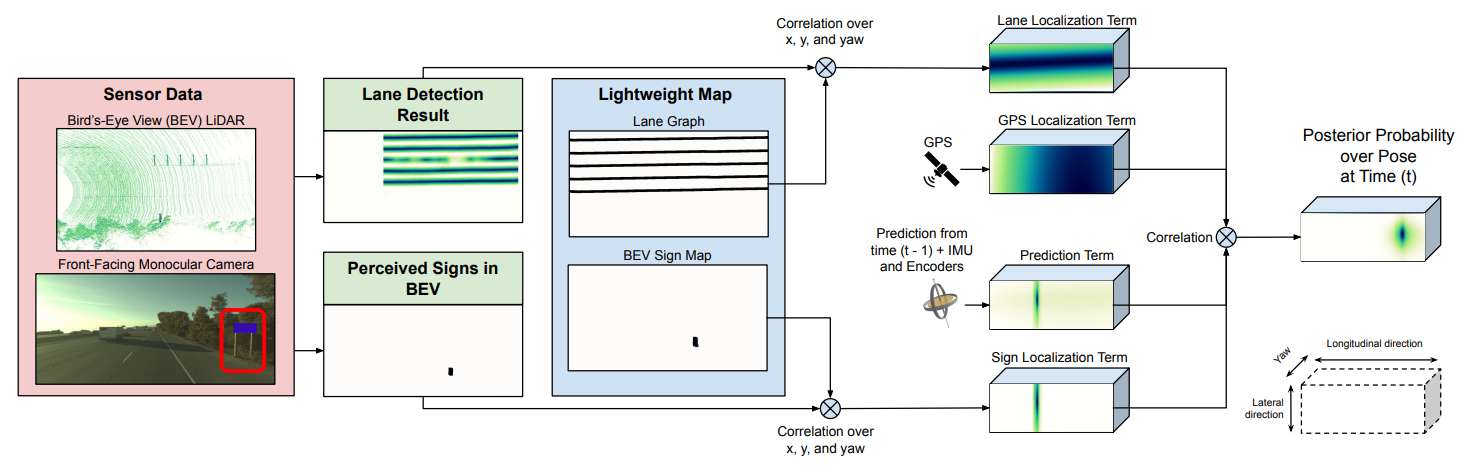
\includegraphics[width=\textwidth]{images/uber_sparse_localization.png}\\
\footnotesize{Localization on a sparse lane and traffic sign map on highways \cite{Ma2019}}
\end{frame}

\begin{frame}
\frametitle{Prediction}
Predicting the future trajectory of traffic is one of the core challenges in
advancing the performance of autonomous vehicles.\\
\vspace{0.25cm}
\centering
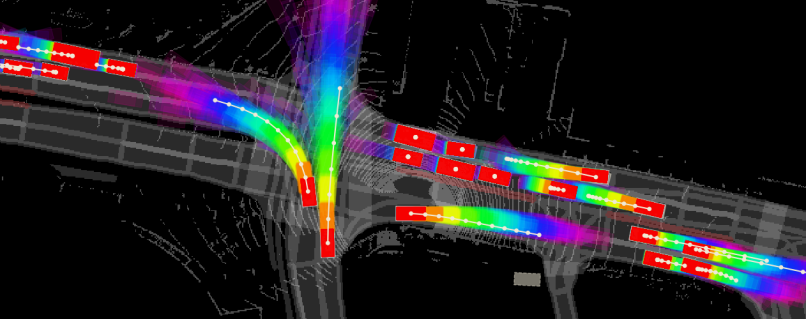
\includegraphics[width=0.8\textwidth]{images/uber_prediction.png}\\
\vspace{0.2cm}
\footnotesize{Heat map of future locations of traffic over time
      (white line is actual trajectory) \cite{Casas2020}}
\end{frame}

\begin{frame}
\frametitle{Motion Planning}
Based on the perception, localization and prediction input, motion planning
plans a safe trajectory for the vehicle to follow. Sampling-based and
optimization methods are the most common approaches.\\
\centering
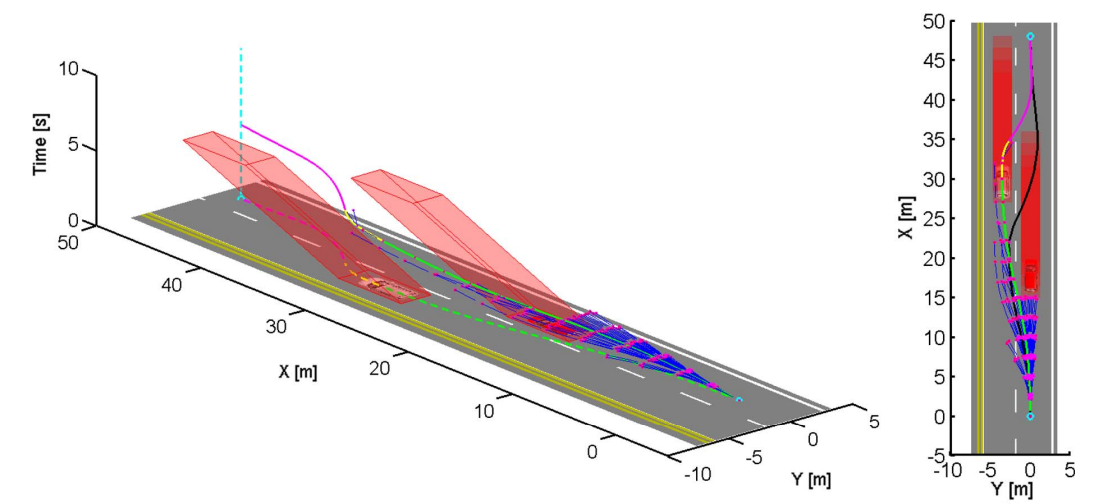
\includegraphics[width=0.8\textwidth]{images/ma_motionplanning.png}\\
\footnotesize{Motion planning in a highway scenario \cite{Ma2015}}
\end{frame}

\subsection{Machine Learning}

\begin{frame}
\frametitle{Machine Learning in Autonomous Driving}
Recent advances in machine learning, in particular deep neural networks, have
affected the algorithmic approach in almost all components in an AV stack.
\begin{columns}[]
    \begin{column}{0.4\textwidth}
        \begin{itemize}
            \item Algorithms are not designed, but models are rather learned
                from (labeled) data
            \item Performance of certain tasks, in particular with computer
                vision, have made major leaps forward
            \item Requires large amount of data
            \item Requires specialized hardware for efficient, real-time 
                processing
        \end{itemize}
    \end{column}
    \begin{column}{0.6\textwidth}
        \centering
        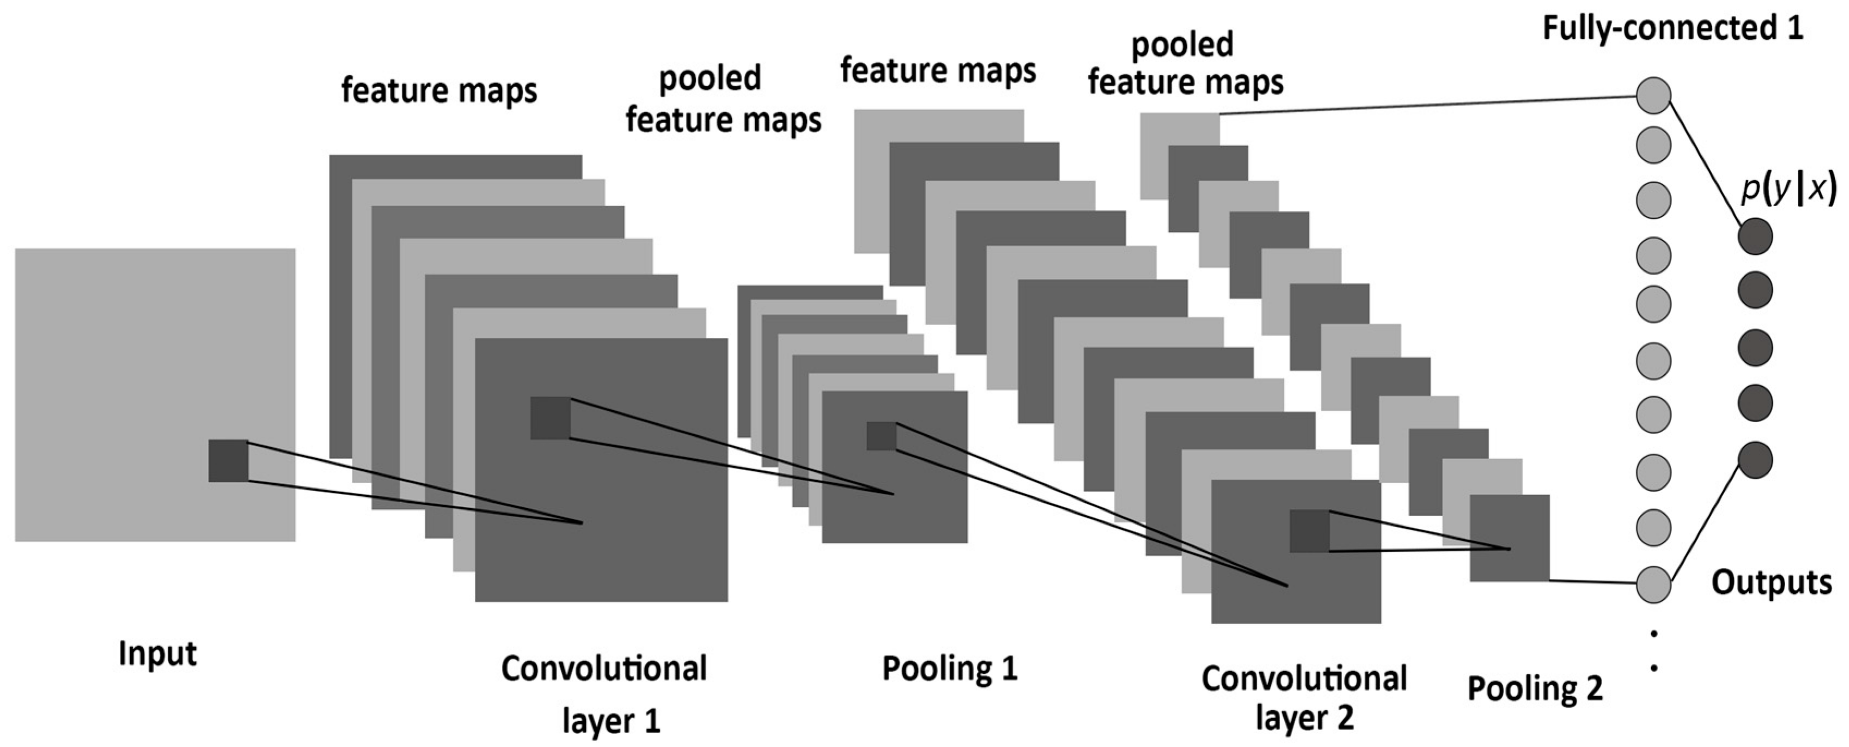
\includegraphics[width=\textwidth]{images/cnn_architecture.png}\\
        \footnotesize{Convolutional neural network architecture for image classification \cite{Albelwi2017}}
    \end{column}
\end{columns}
\end{frame}

\begin{frame}
\frametitle{Machine Learning in Autonomous Driving}
\framesubtitle{Examples for camera sensors}
\begin{columns}[]
    \begin{column}{0.6\textwidth}
        \centering
        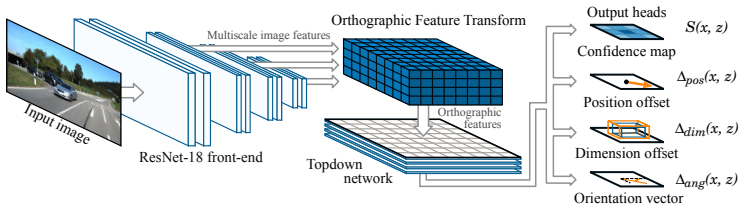
\includegraphics[width=\textwidth]{images/roddick_3d_camera_network.png}\\
        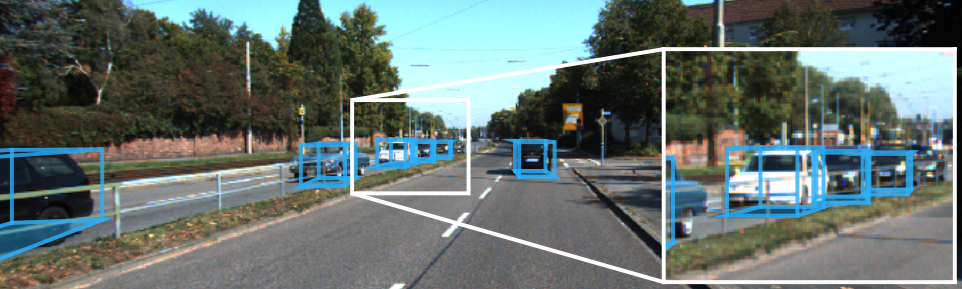
\includegraphics[width=\textwidth]{images/roddick_3d_camera_detections.png}\\
        \vspace{0.1cm}
        \footnotesize{3D camera object detection \cite{Roddick2019}}
    \end{column}
    \begin{column}{0.4\textwidth}
        \centering
        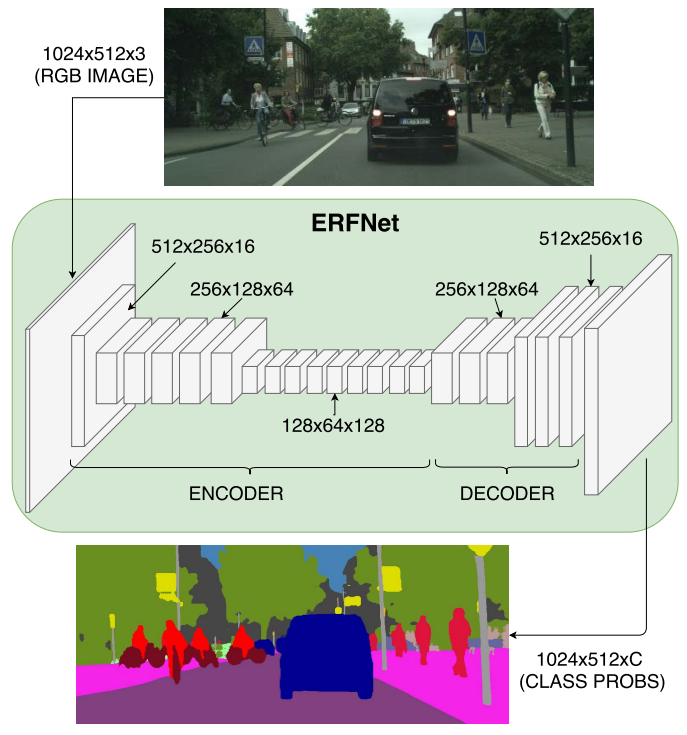
\includegraphics[width=0.9\textwidth]{images/erfnet_semantic_segmentation.png}\\
        \footnotesize{Semantic segmentation \cite{Romera2018}}
    \end{column}
\end{columns}
\end{frame}

\begin{frame}
\frametitle{Machine Learning in Autonomous Driving}
\framesubtitle{Examples for lidar sensors}
\centering
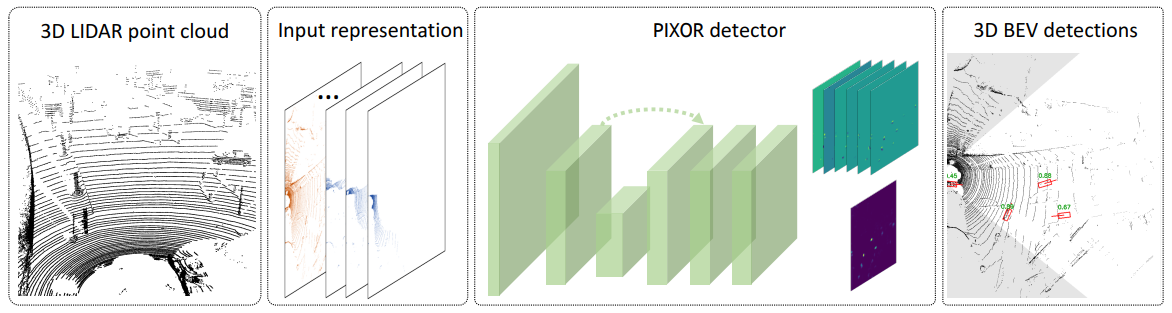
\includegraphics[width=\textwidth]{images/pixor_lidar_object_detection.png}\\
\footnotesize{3D lidar object detection \cite{Yang2018}}
\end{frame}

\begin{frame}
\frametitle{Machine Learning in Autonomous Driving}
\framesubtitle{Examples for lidar sensors}
\centering
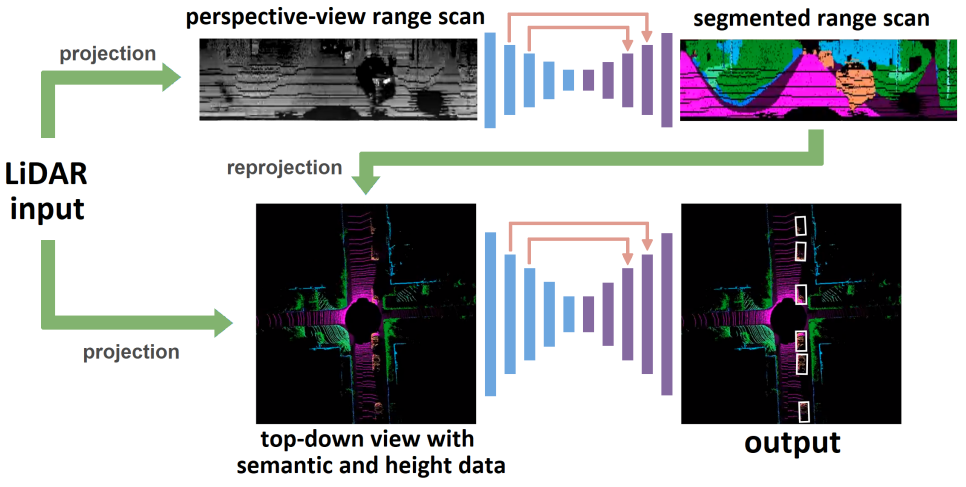
\includegraphics[width=0.8\textwidth]{images/nvidia_lidar_semantic_segmentation.png}\\
\vspace{0.2cm}
\footnotesize{Lidar semantic segmentation \cite{Chen2020}}
\end{frame}

\begin{frame}
\frametitle{Machine Learning in Autonomous Driving}
\framesubtitle{Examples for sensor data fusion}
Deep neural networks can take several sensors as input to realize a learned
approach to sensor data fusion.\\
\vspace{0.25cm}
\centering
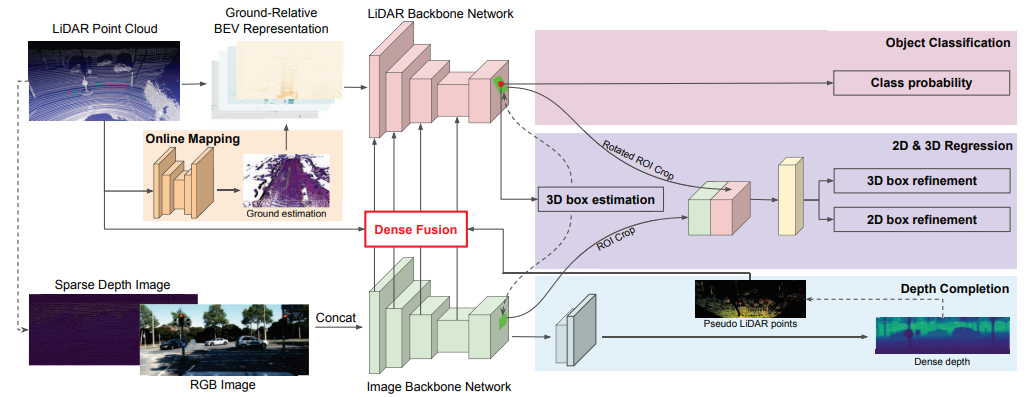
\includegraphics[width=0.9\textwidth]{images/uber_dnn_sensor_fusion.png}\\
\vspace{0.1cm}
\footnotesize{DNN with combined training of lidar and camera \cite{Liang2019}}
\end{frame}

\begin{frame}
\frametitle{Machine Learning in Autonomous Driving}
\framesubtitle{Example for planning components}
ChauffeurNet is an example of deep neural networks directly driving the vehicle
and learning the tasks of prediction and planning.\\
\begin{columns}[T]
    \begin{column}{0.4\textwidth}
        \centering
        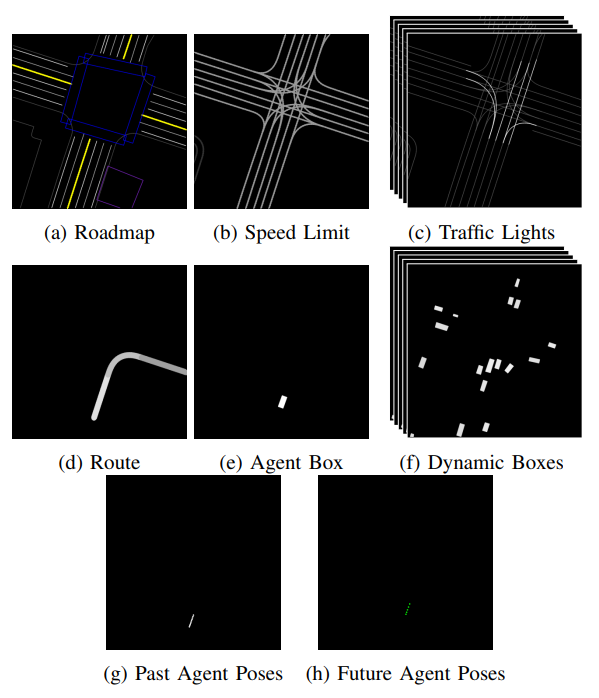
\includegraphics[width=0.7\textwidth]{images/waymo_chauffeurnet_inputs.png}\\
    \end{column}
    \begin{column}{0.6\textwidth}
        \centering
        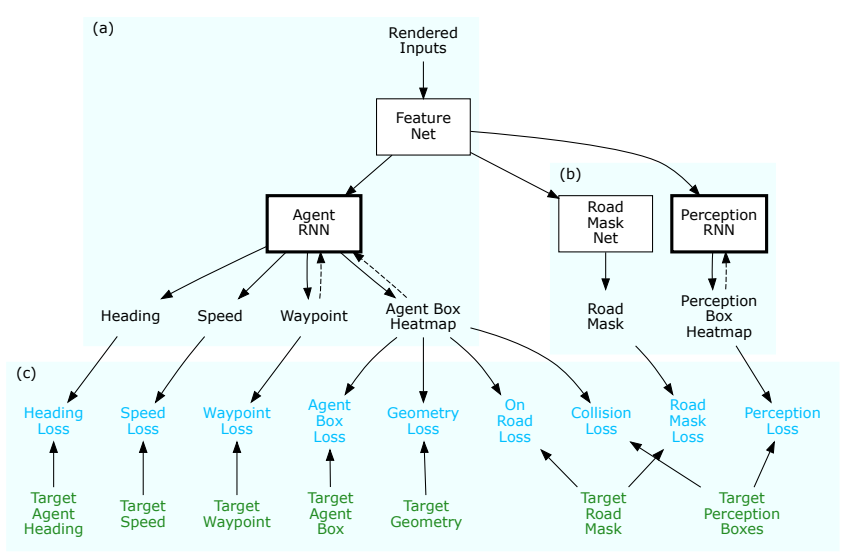
\includegraphics[width=0.8\textwidth]{images/waymo_chauffeurnet_network.png}\\
    \end{column}
\end{columns}
\vspace{0.2cm}
\centering
\footnotesize{ChauffeurNet input images and training architecture \cite{Bansal2019}}
\end{frame}

\subsection{Additional Topics}

\begin{frame}
\frametitle{Architecture for Safety}
A key challenge in autonomous driving is designing a functional architecture
which is robust to failures.

\begin{columns}[T]
    \begin{column}{0.35\textwidth}
        \centering
        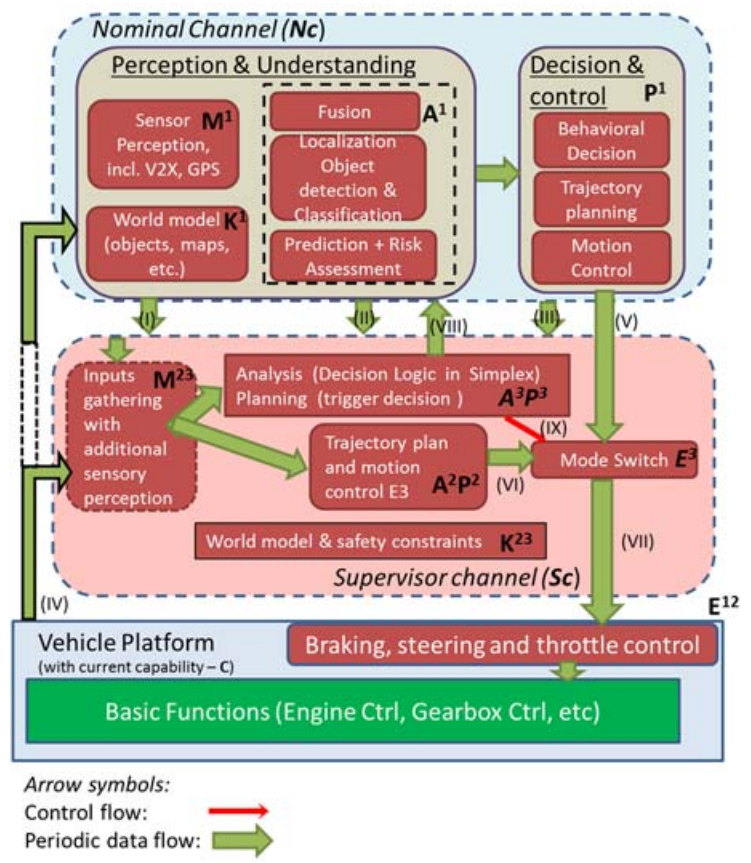
\includegraphics[width=0.95\textwidth]{images/redundant_architecture.png}\\
        \vspace{0.2cm}
        \tiny{Redundant supervisor channel \cite{Torngren2018}}
    \end{column}
    \begin{column}{0.65\textwidth}
        \begin{itemize}
            \item Some form of functional redundancy is required
            \item The redundant system is usually simpler and focuses only on
                safety goals, e.g. collision avoidance
            \item Overrides main system or applies constraints
        \end{itemize}
        \centering
        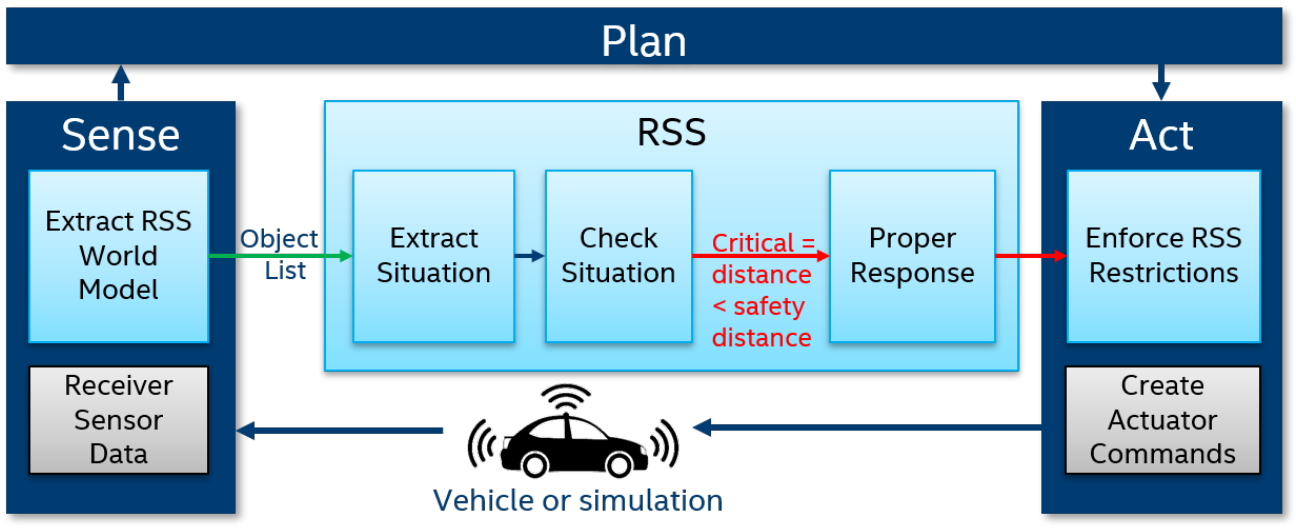
\includegraphics[width=0.75\textwidth]{images/intel_rss.png}\\
        \vspace{0.15cm}
        \tiny{Responsibility Sensitive Safety from Intel/MobilEye \cite{IntelRSS}}
    \end{column}
\end{columns}
\end{frame}

% \begin{frame}
% \frametitle{Datasets}

% \end{frame}

% \begin{frame}
% \frametitle{Books}

% \end{frame}

\section{Software Architecture}

\begin{frame}
\frametitle{Software Architecture}
The implementation of a functional architecture must consider several layers
of software architecture, where many implementation details affect the
performance of the system.\\
\vspace{0.1cm}
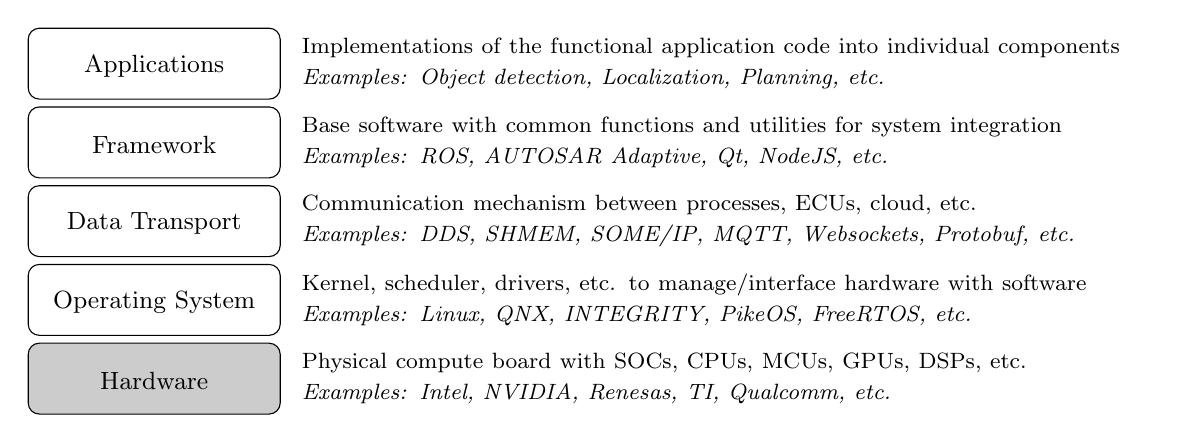
\begin{tikzpicture}[node distance=1cm,font=\small,
    layer/.style={
        draw=black,
        fill=white,
        rounded corners,
        minimum width=3.2cm,
        minimum height=0.9cm,
        text centered,
        text height=8pt},
    layerdark/.style={layer, fill=gray!40},
    ]
    \node[layer] (Apps) {Applications};
    \node[layer, below of=Apps] (FW) {Framework};
    \node[layer, below of=FW] (MW) {Data Transport};
    \node[layer, below of=MW] (OS) {Operating System};
    \node[layerdark, below of=OS] (HW) {Hardware};
    \node (AppsDesc) [right of=Apps, text width=10.75cm, xshift=6.25cm]{
        \footnotesize
        Implementations of the functional application code into individual
        components\\
        \emph{Examples: Object detection, Localization, Planning, etc.}
    };
    \node[right of=FW, text width=10.75cm, xshift=6.25cm] (FWDesc) {
        \footnotesize
        Base software with common functions and utilities for
        system integration\\
        \emph{Examples: ROS, AUTOSAR Adaptive, Qt, NodeJS, etc.}
    };
    \node[right of=MW, text width=10.75cm, xshift=6.25cm] (MWDesc) {
        \footnotesize
        Communication mechanism between processes, ECUs, cloud, etc.\\
        \emph{Examples: DDS, SHMEM, SOME/IP, MQTT, Websockets, Protobuf, etc.}
    };
    \node[right of=OS, text width=10.75cm, xshift=6.25cm] (OSDesc) {
        \footnotesize
        Kernel, scheduler, drivers, etc. to manage/interface hardware with
        software\\
        \emph{Examples: Linux, QNX, INTEGRITY, PikeOS, FreeRTOS, etc.}
    };
    \node[right of=HW, text width=10.75cm, xshift=6.25cm] (HWDesc) {
        \footnotesize
        Physical compute board with SOCs, CPUs, MCUs, GPUs, DSPs, etc.\\
        \emph{Examples: Intel, NVIDIA, Renesas, TI, Qualcomm, etc.}
    };
\end{tikzpicture}
\end{frame}

\begin{frame}
\frametitle{Software Frameworks for Autonomous Driving}
\framesubtitle{Framework requirements}
What are some of the functions, utilities and APIs that an application requires?
\vspace{0.25cm}
\begin{itemize}
    \item Concept of partitioning a larger system into components
    \item Means of receiving and transmitting data between components
    \item Configuration / parametrization of components
    \item Management of component execution und underlying CPU resources,
        e.g. threads
    \item Tools for development, debugging, and deployment
    \item Compatible with different programming languages and platforms
\end{itemize}
\end{frame}

\begin{frame}
\frametitle{Software Frameworks for Autonomous Driving}
\framesubtitle{Today's most popular solutions}
\centering
\begin{columns}[]
    \begin{column}{0.33\textwidth}
        \centering
        
\includegraphics[width=0.8\textwidth]{images/logo_ros.png}\\
    \end{column}
    \begin{column}{0.33\textwidth}
        \centering
        
\includegraphics[width=0.9\textwidth]{images/logo_mathworks.jpg}\\
    \end{column}
    \begin{column}{0.33\textwidth}
        \centering
        
\includegraphics[width=0.3\textwidth]{images/logo_elektrobit.jpg}\\
    \end{column}
\end{columns}
\vspace{0.2cm}
\begin{columns}[]
    \begin{column}{0.33\textwidth}
        \centering
        \footnotesize
        Robot Operating System\footnotemark[1]\\
    \end{column}
    \begin{column}{0.33\textwidth}
        \centering
        \footnotesize
        MATLAB/Simulink\footnotemark[2]
    \end{column}
    \begin{column}{0.33\textwidth}
        \centering
        \footnotesize
        EB Assist ADTF\footnotemark[3]
    \end{column}
\end{columns}
\vspace{0.25cm}
\begin{columns}[]
    \begin{column}{0.33\textwidth}
        \centering
        
\includegraphics[width=0.9\textwidth]{images/logo_autosar.png}\\
    \end{column}
    \begin{column}{0.33\textwidth}
        \centering
        
\includegraphics[width=0.6\textwidth]{images/logo_nvidia.png}\\
    \end{column}
    \begin{column}{0.33\textwidth}
        \centering
        
\includegraphics[width=0.8\textwidth]{images/logo_motionwise.png}\\
    \end{column}
\end{columns}
\vspace{0.2cm}
\begin{columns}[]
    \begin{column}{0.33\textwidth}
        \centering
        \footnotesize
        AUTOSAR\footnotemark[4]
    \end{column}
    \begin{column}{0.33\textwidth}
        \centering
        \footnotesize
        NVIDIA DriveWorks\footnotemark[5]
    \end{column}
    \begin{column}{0.33\textwidth}
        \centering
        \footnotesize
        TTTech Auto MotionWise\footnotemark[6]
    \end{column}
\end{columns}
\footnotetext[1]{\tiny{\url{https://ros.org/}}}
\footnotetext[2]{\tiny{\url{https://www.mathworks.com/products/automated-driving.html}}}
\footnotetext[3]{\tiny{\url{https://www.elektrobit.com/products/automated-driving/eb-assist/adtf/}}}
\footnotetext[4]{\tiny{\url{https://www.autosar.org/}}}
\footnotetext[5]{\tiny{\url{https://developer.nvidia.com/drive/driveworks}}}
\footnotetext[6]{\tiny{\url{https://www.tttech-auto.com/products/safety-software-platform/motionwise/}}}
\end{frame}

\begin{frame}
\frametitle{Software Frameworks for Autonomous Driving}
\framesubtitle{Today's most popular solutions}
\begin{center}
    
\includegraphics[width=0.4\textwidth]{images/logo_apexai.png}
\end{center}
\vspace{0.25cm}
Apex.AI\footnotemark[1] has developed Apex.OS\footnotemark[2] and
Apex.Middleware\footnotemark[3], a software framework and
middleware based on ROS and designed for safety-certified automotive
applications.
\footnotetext[1]{\tiny{\url{https://www.apex.ai/}}}
\footnotetext[2]{\tiny{\url{https://www.apex.ai/apex-os}}}
\footnotetext[3]{\tiny{\url{https://www.apex.ai/apex-middleware}}}
\end{frame}

\subsection{ROS}

\begin{frame}
\frametitle{Robot Operating System (ROS)}
\framesubtitle{Overview}
\begin{columns}[]
    \begin{column}{0.7\textwidth}
        \begin{itemize}
            \item Most popular framework for developing robotics (and other)
                applications
            \item Open source with thousands of contributors world wide
            \item Widely adopted by universities, research institutes and
                and companies
            \item Thousands of packages\footnotemark[1] (applications) for
                sensors, perception, SLAM, motion planning, etc.
            \item Powerful suite of tools (visualization, introspection,
                debugging, etc.)
            \item Wide support for different programming languages
            \item Hundreds of autonomous vehicles in R\&D run on ROS
        \end{itemize}
    \end{column}
    \begin{column}{0.3\textwidth}
        \centering
        \includegraphics[width=\textwidth]{images/logo_ros.png}
    \end{column}
\end{columns}
\footnotetext[1]{\tiny{\url{https://index.ros.org/packages/}}}
\end{frame}

\begin{frame}
\frametitle{Robot Operating System (ROS)}
\framesubtitle{The basics}
\begin{columns}[]
    \begin{column}{0.5\textwidth}
        \begin{itemize}
            \item \textbf{Nodes}: A single processing entity with inputs and
                outputs
            \item \textbf{Topics}: Data channels between nodes
            \item \textbf{Messages}: The data type which is transmitted on a
                topic
            \item \textbf{Publisher}: Within a node, the entity that transmits
                data on a topic
            \item \textbf{Subscriber}: Within a node, the entity that receives
                data on a topic
            \item \textbf{Service}: Request/response mechanism between nodes
        \end{itemize}
    \end{column}
    \begin{column}{0.5\textwidth}
        \centering
        \includegraphics[width=\textwidth]{images/ros_overview.png}
        \tiny{Source: ROS 2 Tutorials - Understanding ROS 2 nodes\footnotemark[1]}
    \end{column}
\end{columns}
\footnotetext[1]{\tiny{\url{https://docs.ros.org/en/galactic/Tutorials/Understanding-ROS2-Nodes.html}}}
\end{frame}

\begin{frame}[fragile]
\frametitle{Robot Operating System (ROS)}
\framesubtitle{Example ROS 2 node in C++}
\tiny
\begin{minted}{cpp}
// From https://docs.ros.org/en/galactic/Tutorials/Writing-A-Simple-Cpp-Publisher-And-Subscriber.html
class MinimalPublisher : public rclcpp::Node {
    public:
        MinimalPublisher() : Node("minimal_publisher"), count_(0) {
            publisher_ = this->create_publisher<std_msgs::msg::String>("topic", 10);
            timer_ = this->create_wall_timer(500ms, std::bind(&MinimalPublisher::timer_callback, this));
        }
    private:
        void timer_callback() {
            auto message = std_msgs::msg::String();
            message.data = "Hello, world! " + std::to_string(count_++);
            RCLCPP_INFO(this->get_logger(), "Publishing: '%s'", message.data.c_str());
            publisher_->publish(message);
        }
        rclcpp::TimerBase::SharedPtr timer_;
        rclcpp::Publisher<std_msgs::msg::String>::SharedPtr publisher_;
        size_t count_;
};

int main(int argc, char * argv[]) {
    rclcpp::init(argc, argv);
    rclcpp::spin(std::make_shared<MinimalPublisher>());
    rclcpp::shutdown();
    return 0;
}
\end{minted}
\end{frame}

\begin{frame}
\frametitle{Robot Operating System (ROS)}
\framesubtitle{Tools}
\begin{columns}[]
    \begin{column}{0.65\textwidth}
        \footnotesize
        ROS has a rich suite of tools, both included in the standard installation as
        well as tools developed by the community.\\
        \begin{itemize}
            \item Command line tools for system introspection, configuration,
                and launching
            \item rosbag\footnotemark[1] recording and replay tool
            \item RViz\footnotemark[2]: 3D Visualizer
            \item rqt\footnotemark[3]: Qt based GUI with customizable plug-ins
            \item Robot Web Tools\footnotemark[4]: web based interfacing with ROS
            \item PlotJuggler\footnotemark[5]: plotting of ROS message data 
        \end{itemize}
    \end{column}
    \begin{column}{0.35\textwidth}
        \centering
        \includegraphics[width=0.6\textwidth]{images/rviz.jpg}\\
        \scriptsize RViz\footnotemark[2] 3D Visualizer\\
        Source: YouTube (Autoware)\footnotemark[6]\\
        \vspace{0.25cm}
        \includegraphics[width=0.6\textwidth]{images/rqt.png}\\
        \scriptsize rqt\footnotemark[3] GUI
    \end{column}
\end{columns}
\footnotetext[1]{\tiny{\url{https://github.com/ros2/rosbag2}}}
\footnotetext[2]{\tiny{\url{https://github.com/ros2/rviz}}}
\footnotetext[3]{\tiny{\url{http://wiki.ros.org/rqt}}}
\footnotetext[4]{\tiny{\url{http://robotwebtools.org/}}}
\footnotetext[5]{\tiny{\url{https://www.plotjuggler.io/}}}
\footnotetext[6]{\tiny{\url{https://www.youtube.com/watch?v=zujGfJcZCpQ}}}
\end{frame}

\subsection{Production Frameworks}

\begin{frame}
\frametitle{Production Software Frameworks}
A software framework and middleware for a production vehicle has many
additional requirements that need to be met.

\begin{itemize}
    \item Safety requirements and standards must be met
    \item Software must run on embedded hardware with limited resources
    \item Automotive interfaces must be supported (CAN, LIN, automotive
        Ethernet, etc.)
    \item Security requirements must be met, e.g. end-to-end protection, 
        identity access management, etc.
    \item Automotive interfaces such as Unified Diagnostics Service (UDS) must
        be implemented
\end{itemize}
\end{frame}

\begin{frame}
\frametitle{AUTOSAR Classic}
AUTOSAR was formed in 2003 to standardize automotive E/E architecture.
Applications can be developed against a standard Runtime Environment
for automotive \emph{microcontrollers}.
\begin{center}
\includegraphics[width=0.75\textwidth]{images/autosar_classic.png}\\
\footnotesize  Source: AUTOSAR Classic Platform\footnotemark[1]
\end{center}
\footnotetext[1]{\tiny{\url{https://www.autosar.org/standards/classic-platform/}}}
\end{frame}

\begin{frame}
\frametitle{AUTOSAR Adaptive}
Next-generation of AUTOSAR designed for high performance computing hardware
running with a POSIX based operating system. Uses a service oriented
architecture.
\begin{center}
\includegraphics[width=0.7\textwidth]{images/autosar_adaptive.png}\\
\footnotesize Source: AUTOSAR Classic Platform\footnotemark[1]
\end{center}
\footnotetext[1]{\tiny{\url{https://www.autosar.org/standards/adaptive-platform/}}}
\end{frame}

\begin{frame}
\frametitle{Apex.OS}
Apex.OS is a production framework and SDK based on ROS 2.
\begin{center}
\includegraphics[width=\textwidth]{images/apex_ros_to_apexos.png}\\
\scriptsize Source: Apex.AI
\end{center}
\end{frame}

\subsection{Middleware}

\begin{frame}
\frametitle{Data Transport Middlewares}
\framesubtitle{Overview}
A complete vehicle system requires many different mechanism for transporting
data from one component to another.\\
\begin{columns}[]
    \begin{column}{0.6\textwidth}
        Middleware requirements:
        \begin{itemize}
            \item Handle GByte/s data transfer (e.g. camera images)
            \item Short latencies and low run-time resource consumption
            \item Many-to-many communication
            \item Interfacing with diverse set of protocols
        \end{itemize}
    \end{column}
    \begin{column}{0.4\textwidth}
        \centering
        \includegraphics[width=\textwidth]{images/apex_vehicle_coms.png}\\
        \scriptsize Source: Apex.AI
    \end{column}
\end{columns}
\end{frame}

\begin{frame}
\frametitle{Data Transport Middlewares}
\framesubtitle{Automotive communication buses}
Automotive communication mechanisms are designed to be robust and reliable
where several ECUs can exchange data.
\begin{itemize}
    \item CAN: Reliable bus system to exchange small bits of data across many ECUs
    \item FlexRay: Improved performance for safety-critical systems
    \item LIN: Integration of simple sensors and actuators
    \item MOST: Designed for the transmission of multimedia data,
        e.g. video, audio, etc.
    \item Ethernet: High-bandwidth data exchance based on IP networking
\end{itemize}
For each of these technologies, a middleware software stack is required to make
the data on the bus system available to an application. In the automotive
industry, this is often accomplished with the AUTOSAR Classic stack.
\end{frame}

\justfor{long}{
\begin{frame}
\frametitle{Data Transport Middlewares}
\framesubtitle{Ethernet}
In recent years, automotive Ethernet has made it into production vehicles,
enabling the high-bandwidth data rates of Ethernet with the well-known
TCP and UDP networking protocols. Two popular software middlewares are built
on Ethernet.
\begin{columns}[T]
    \begin{column}{0.5\textwidth}
        \includegraphics[width=0.125\textwidth]{images/dds.jpg}
        \begin{itemize}
            \item DDS\footnotemark[1] is an OMG standard
            \item Publisher/subscriber on topics
            \item Standardized interface, OMG IDL\footnotemark[2]
            \item Rich set quality of service settings
            \item Used in many industries: automotive, robotics, banking,
                medical, aerospace
        \end{itemize}
    \end{column}
    \begin{column}{0.5\textwidth}
        SOME/IP\footnotemark[3]\\
        \begin{itemize}
            \item Standardized within the scope of AUTOSAR \cite{AutosarSomeIp}
            \item Service oriented architecture
            \item Interface definition with ARXML (from AUTOSAR)
            \item No quality of service
            \item Mainly used in automotive
        \end{itemize}
    \end{column}
\end{columns}
\footnotetext[1]{\tiny{\url{https://www.dds-foundation.org/}}}
\footnotetext[2]{\tiny{\url{https://www.omg.org/spec/IDL/4.2/About-IDL/}}}
\footnotetext[3]{\tiny{\url{https://some-ip.com/}}}
\end{frame}
}

\begin{frame}
\frametitle{Data Transport Middlewares}
\framesubtitle{Shared memory}
For data transmission of high-bandwidth data (e.g. camera data) on the same
ECU, the copying, serialization, and deserialization of the data consumes
significant CPU resources.\\

An efficient shared memory data transport is required to reduce the CPU
overhead. The Eclipse iceoryx\texttrademark\footnotemark[1] shared memory
middleware enables constant-time true zero-copy data transport.

\begin{center}
\includegraphics[width=0.5\textwidth]{images/shared_memory.png}\\
\footnotesize Source: Eclipse Foundation\footnotemark[1]
\end{center}
\footnotetext[1]{\tiny{\url{https://www.eclipse.org/community/eclipse_newsletter/2019/december/4.php}}}
\end{frame}

\justfor{long}{
\begin{frame}
\frametitle{Data Transport Middlewares}
\framesubtitle{Apex.Middleware}
\begin{columns}[]
    \begin{column}{0.6\textwidth}
        A single middleware designed to communicate using different protocols
        in the context of automotive and robotics applications.
        \begin{itemize}
            \item Shared memory backbone with Eclipse iceoryx\texttrademark\footnotemark[1]
            \item Ethernet communication with Eclipse Cyclone DDS\texttrademark\footnotemark[2]
                and automotive SOME/IP
            \item Support for PDU communication, e.g. CAN
            \item MQTT for cloud connectivity
        \end{itemize}
    \end{column}
    \begin{column}{0.4\textwidth}
        \centering
        \includegraphics[width=0.8\textwidth]{images/apex_middleware.png}\\
        \scriptsize Source: Apex.AI
    \end{column}
\end{columns}
\footnotetext[1]{\tiny{\url{https://iceoryx.io/}}}
\footnotetext[2]{\tiny{\url{https://cyclonedds.io/}}}
\end{frame}
}

\subsection{Operating Systems}

\begin{frame}
\frametitle{Operating Systems}
The operating system is responsible for managing the interface between software
applications and the underlying hardware: memory management, process/task
management, input/output communications, etc.
\begin{columns}[]
    \begin{column}{0.7\textwidth}
        \begin{itemize}
            \item Modern high-performance computers run a
                POSIX compliant (real-time) operating system (Linux, QNX$^{\tiny{\textregistered}}$,
                INTEGRITY, PikeOS, etc.)
            \item AUTOSAR Classic OSEK \cite{ISO17356} dominates the automotive microcontrollers
            \item A Hypervisor can be used to manage several guest operating systems
                sharing the resources of a single CPU
                \begin{itemize}
                    \item Partitioning of safety and non-safety applications
                \end{itemize}
            \item Development is typically on Linux or Windows
        \end{itemize}
    \end{column}
    \begin{column}{0.3\textwidth}
        \centering
        \includegraphics[height=2cm]{images/linux-logo.png}\\
        \scriptsize Source: Wikipedia\footnotemark[1]\\
        \vspace{0.5cm}
        \includegraphics[width=0.9\textwidth]{images/qnx-logo.png}\\
        \scriptsize Source: Blackberry QNX$^{\tiny{\textregistered}}$\footnotemark[2]
    \end{column}
\end{columns}
\footnotetext[1]{\tiny{\url{https://en.wikipedia.org/wiki/Linux}}}
\footnotetext[2]{\tiny{\url{https://blackberry.qnx.com/en/products/safety-certified/qnx-os-for-safety}}}
\end{frame}
\section{Hardware Architecture}

\begin{frame}
\frametitle{Hardware Architecture}
The hardware used in an autonomous vehicle project evolves with the different
stages of development.

\begin{itemize}
    \item \textbf{Research}: Off-the-shelf hardware (x86 PCs, network switches, etc.) are used
        in early stages of development in order to focus on the functional
        software.
    \item \textbf{Pre-development}: Evaluation boards from chip vendors, or ruggedized version from
        third parties, are often used in pre-development stages to begin
        the work of optimizing the software for an embedded environment.
    \item \textbf{Production}: Hardware is produced in cooperation with a Tier 1
        supplier (e.g. Continental, ZF, Bosch, etc.), where several samples
        (A-sample to D-sample) are produced before the final version is made
        for start of production (SOP).
\end{itemize}
\end{frame}

\begin{frame}
\frametitle{Hardware Architecture}
\framesubtitle{Early prototyping}
Example of an early prototype with off-the-shelf hardware, but also prototype
hardware from automotive vendors (VIGEM, Elektrobit seen here).
\begin{center}
\includegraphics[width=0.5\textwidth]{images/bmw_vehicle_trunk.jpg}\\
\footnotesize Source: BMW\footnotemark[1]
\end{center}
\footnotetext[1]{\tiny{\url{https://www.press.bmwgroup.com/global/article/detail/T0320230EN/nextgen-2020}}}
\end{frame}

\begin{frame}
\frametitle{Hardware Architecture}
\framesubtitle{First embedded hardware}
Developer kits from chip vendors serve as a good platform for doing an initial
integration of a system to an embedded environment and optimizing the
application.
\begin{center}
\includegraphics[width=0.6\textwidth]{images/nvidia_drive_agx.jpg}\\
\footnotesize Source: NVIDIA\footnotemark[1]
\end{center}    
\footnotetext[1]{\tiny{\url{https://developer.nvidia.com/drive/drive-agx}}}
\end{frame}

\begin{frame}
\frametitle{Hardware Architecture}
\framesubtitle{Production hardware}
Tier 1 suppliers develop rugged and automotive grade ECUs for mass production,
often customized for an OEM's specific requirements.\\
\vspace{0.2cm}
\begin{columns}[]
    \begin{column}{0.5\textwidth}
        \centering
        \includegraphics[width=0.7\textwidth]{images/zf_proai_s500l.jpg}\\
        \footnotesize ZF ProAI S500L\footnotemark[1]
    \end{column}
    \begin{column}{0.5\textwidth}
        \centering
        \includegraphics[width=0.7\textwidth]{images/continental_ecu.jpg}\\
        \footnotesize Continental ADAS/AD ECU\footnotemark[2]
    \end{column}
\end{columns}
\footnotetext[1]{\tiny{\url{https://www.zf.com/products/en/cars/stories/proai.html}}}
\footnotetext[2]{\tiny{\url{https://www.continental-automotive.com/en-gl/Passenger-Cars/Autonomous-Mobility/Enablers/Control-Units/Assisted-Automated-Driving-Control-Unit}}}
\end{frame}

\begin{frame}
\frametitle{Hardware Architecture}
\framesubtitle{Designing for safety and performance}
A single, modern ECU designed to be a central domain controller for a vehicle
may contain several different processing units to achieve the overall goals
of safety and performance.

\begin{itemize}
    \item CPUs at the core of the computing, mostly ARM-based architectures
    \item Hardware accelerators for specific tasks: GPUs, DSPs, NPUs, etc.
    \item Customized computing: ASICs, FPGAs
    \item Safety-critical microcontrollers
    \item SPI, Ethernet, PCI Express, hardware shared memory, etc. for
        communication between computing cores
    \item SOCs may combines several types of computing cores onto a single chip
\end{itemize}
\end{frame}

\begin{frame}
\frametitle{Hardware Architecture}
\framesubtitle{Current 4th-Gen architectures and future 5th-Gen architectures}
\small{Automotive vehicle-wide ECU architectures are evolving and undergoing
drastic changes. Hardware complexity is being reduced by integrating fewer,
but more powerful, ECUs.}
%\vspace{0.1cm}
\begin{columns}[]
    \begin{column}{0.6\textwidth}
        \centering
        \includegraphics[width=0.65\textwidth]{images/mckinsey_vehicle_architecture_generations.png}\\
        \tiny Evolution from 3rd Gen to 5th Gen architectures \cite{McKinseyReport}
    \end{column}
    \begin{column}{0.4\textwidth}
        \centering
        \includesvg[svgextension=svgz,height=0.55\textheight]{images/mckinsey_hw_architecture_5th_gen_zonal.svgz}\\
        \tiny{5th Gen Zonal Architecture\footnotemark[1]}
    \end{column}
\end{columns}
\footnotetext[1]{\tiny{\url{https://www.mckinsey.com/industries/automotive-and-assembly/our-insights/rewiring-car-electronics-and-software-architecture-for-the-roaring-2020s}}}
\end{frame}


\section{Software Engineering}

\subsection{Introduction}

\begin{frame}
\frametitle{Software Engineering}
A core challenge for bringing autonomous driving to market is the sheer scale
of the engineering effort required.
\begin{itemize}
    \item Software must be developed that will scale in terms of complexity
        and the number of developers working on it
    \item Integration, testing and deployment must be efficient, fast and
        reliable
    \item A large number of engineers must be coordinated to work towards a
        single, common goal
    \item Product and development process must comply to a wide range of
        industry standards
\end{itemize}
\pause
\begin{block}{}
These aspects of software engineering are often the majority of the effort 
required for developing a product $\rightarrow$ the functional application
may be simple in comparison.
\end{block}
\end{frame}

\begin{frame}
\frametitle{Software Best Practices}
It is important that the code you write can be easily understood by someone
you may never meet, several years later, long after you've left the project
or company.

\begin{columns}[]
    \begin{column}{0.65\textwidth}
        \begin{itemize}
            \item Practice clean code
            \begin{itemize}
                \item Use human-understandable and meaningful variable/function/class
                    names
                \item Keep method/function size small
                \item The code \emph{is} the documentation
            \end{itemize}
            \item Follow the SOLID and DRY principles
            \item Minimize technical debt
            \item Code reviews are a must
            \item Use coding guidelines and enforce them with linters
        \end{itemize}   
    \end{column}
    \begin{column}{0.35\textwidth}
        \centering
        \includegraphics[height=0.75\textwidth]{images/book_clean_code.jpg}\\
        \footnotesize{\emph{Clean Code} by Robert C. Martin\footnotemark[1]}
    \end{column}
\end{columns}
\footnotetext[1]{\tiny{\url{https://www.oreilly.com/library/view/clean-code-a/9780136083238/}}}
\end{frame}

% \begin{frame}
% \frametitle{Software Best Practices}
% The SOLID principles, introduced by Robert C. Martin, are a great guide
% for designing software that is understandable and maintainable.
% \begin{itemize}
%     \item \textbf{S}ingle-Responsibility Principle: Function/classes/etc.
%         should do only \emph{one} thing.
%     \item \textbf{O}pen-Closed Principle: Entities are open for extension, but
%         closed for modification. 
%     \item \textbf{L}iskov Substitution Principle: If S is a subtype of T, then
%         objects of type T may be replaced with objects of type S
%     \item \textbf{I}nterface Segregation Principle: 
%     \item \textbf{D}ependency Inversion Principle:
% \end{itemize}
% The SOLID principles can also be applied to functional and software
% architecture and design. The Clean Architecture\footnotemark[1] book is a great
% reference.
% \footnotetext[1]{\tiny{\url{https://www.oreilly.com/library/view/clean-architecture-a/9780134494272/}}}
% \end{frame}

\subsection{CI/CD}

\begin{frame}
\frametitle{Continuous Integration / Delivery / Deployment}
Modern software engineering is not feasible without continuous integration and
continuous deployment.\\

\textbf{Continuous Integration}: Automated building, testing, and integration 
with every change in the software.\\

\textbf{Continuous Delivery}: Release artifacts are created and automatically
tested in pre-production environments. Deployment into the field is done
manually.\\

\textbf{Continuous Deployment}: Ability to deploy software into the field
automatically.\\

\pause

\begin{block}{}
What does CI/CD looks like in practice for an autonomous vehicles?
\end{block}
\end{frame}

\begin{frame}
\frametitle{Continuous Integration / Deployment}
\framesubtitle{Pipeline for a fleet of autonomous vehicles}
\includegraphics[width=\textwidth]{images/autonomous_driving_ci-cd_pipeline.png}
% \begin{tikzpicture}[node distance=0.25cm,font=\scriptsize,
%     every node/.style={inner sep=0,outer sep=0},
%     stage/.style={
%         draw=black, fill=white,
%         rounded corners,
%         minimum width=1cm, minimum height=1.2cm,
%         text centered, align=center,
%         inner sep=1mm, outer sep=1mm},
%     release/.style={
%         trapezium,
%         trapezium stretches=true,
%         trapezium left angle=70,
%         trapezium right angle=110,
%         minimum height=1.2cm,
%         text centered, align=center,
%         draw=black, fill=white,
%         inner sep=1mm, outer sep=1mm,
%         anchor=south}
%     ]
%     \node[stage] (build) {Build \&\\Unit Tests};
%     \node[stage, right=of build] (integration) {Integration\\Tests};
%     \node[stage, right=of integration] (acceptance_sil) {Acceptance\\Tests};
%     \node[release, right=of acceptance_sil] (release_candidate) {Release\\Candidate};
%     \node[stage, right=of release_candidate] (hil_acceptance_test) {Acceptance\\Tests};
%     \node[stage, above=of hil_acceptance_test] (hil_nonfunc) {Non-Func.\\Tests};
%     \node[stage, below=of hil_acceptance_test] (hil_integration) {Integration\\Tests};
%     \node[stage, right=of hil_acceptance_test] (test_track) {Test Track\\Testing};
%     \node[stage, right=of test_track, yshift=-0.75cm] (shadow) {Shadow\\Testing};
%     \node[stage, right=of test_track, yshift=0.75cm] (fleet) {Fleet\\Testing};
%     \node[release, right=of shadow] (deploy) {Deploy};
% \end{tikzpicture}
\end{frame}

\begin{frame}
\frametitle{Continuous Integration / Deployment}
\framesubtitle{Example CI/CD pipeline from Apex.AI}
\centering
\includegraphics[height=0.78\textheight]{images/apex_cicd.png}\\
\footnotesize{Source: Apex.AI}
\end{frame}

\subsection{Testing}

\begin{frame}
\frametitle{Testing}
Software testing is a vital aspect of successful software development, in
particular for a safety-relevant application such as autonomous vehicles.

\begin{itemize}
    \item Treat test code to the same standards as production code
    \item The amount of test code will likely be multiple factors larger 
        than the actual production application code
    \item Tests should be automated, repeatable and independent
    \item Test the behavior, not the implementation
    \item Follow Arrange - Act - Assert pattern
    \item The scope of the system under test should be increased with every
        stage of a CI/CD pipeline
\end{itemize}
\end{frame}

\begin{frame}[fragile]
\frametitle{Unit Testing}
Testing of the smallest, simplest entities, e.g. classes, functions, etc.\\
\begin{columns}[]
    \begin{column}{0.5\textwidth}
        \begin{itemize}
            \item Tests are lightning fast
            \item Number of tests is incredibly large
            \item Tests have no external dependencies (e.g. to file system, etc.)
            \item Test expected failure cases, e.g. invalid input
            \item GoogleTest\footnotemark[1] for C++
        \end{itemize}
    \end{column}
    \begin{column}{0.5\textwidth}
\tiny
\begin{minted}{cpp}
TEST(VehicleSpeedChecks, IsVehicleOverSpeedLimit)
{
    // Arrange
    constexpr float vehicle_speed_kmh = 120;
    constexpr float speed_limit_kmh = 100;

    // Act
    auto speeding =
        isVehicleSpeeding(vehicle_speed_kmh, speed_limit_kmh);

    // Assert
    EXPECT_TRUE(speeding);
}
\end{minted}
    \end{column}
\end{columns}
\begin{exampleblock}{Example for autonomous vehicles}
Individual functions from a Kalman filter library, e.g. predict(), are tested.
\end{exampleblock}
\footnotetext[1]{\tiny{\url{https://github.com/google/googletest}}}
\end{frame}

\begin{frame}
\frametitle{Integration Testing}
Multiple components of a system are tested together.
\begin{itemize}
    \item Black-box testing (implementation details of components are not known)
    \item Tests interfaces and interactions between components
    \item Input is more complex
    \item Tests may run longer and take more resources
    \item May interact with external dependencies, e.g. file system
    \item In ROS, the launch\_testing\footnotemark[1] framework can be used to
        do integration testing on a system of nodes
\end{itemize}
\begin{exampleblock}{Example for autonomous vehicles}
A lidar perception pipeline is tested, e.g. the components of clustering and
tracking are tested together.
\end{exampleblock}
\footnotetext[1]{\tiny{\url{https://github.com/ros2/launch/tree/master/launch_testing}}}
\end{frame}

\begin{frame}
\frametitle{Acceptance Testing}
Testing the overall product behavior based on functional and business
requirements.
\begin{itemize}
    \item Validates the product requirements
    \item Requires interaction between product/business and engineering
    \item Simulations or recorded data can be used as input
    \item Given - When - Then pattern
    \item Cucumber\footnotemark[1] framework
    \item Often called \emph{Scenario-based Testing} in the autonomous vehicles
        space
\end{itemize}
\begin{center}
\includegraphics[width=0.42\textwidth]{images/carla_simulation.png}\\
\footnotesize{CARLA open source simulator for autonomous driving \cite{Dosovitskiy17}}
\end{center}
\begin{exampleblock}{Example for autonomous vehicles}
The vehicle behaves correctly when approaching a red light.
\end{exampleblock}
\footnotetext[1]{\tiny{\url{https://cucumber.io/}}}
\end{frame}

\begin{frame}
\frametitle{Manual Acceptance Testing}
\begin{columns}[]
    \begin{column}{0.55\textwidth}
        Some acceptance testing is impossible, or very difficult, to automate,
        which still requires some testing to be done manually.\\
        \begin{itemize}
            \item Interaction with users is required, e.g. user acceptance testing
            \item System under test is increased to include artifacts of the
                physical, which cannot be automated in computer systems
        \end{itemize}
    \end{column}
    \begin{column}{0.45\textwidth}
        \centering
        \includegraphics[width=0.8\textwidth]{images/m-city.jpg}\\
        \footnotesize{Mcity Test Facility at University of Michigan\footnotemark[1]}
    \end{column}
\end{columns}
\begin{exampleblock}{Example for autonomous vehicles}
In-vehicle testing with a safety-driver, either on the test track or with a
fleet on public roads.
\end{exampleblock}
\footnotetext[1]{\tiny{\url{https://mcity.umich.edu/our-work/mcity-test-facility/}}}
\end{frame}

\begin{frame}
\frametitle{Test-Driven Development}
Methodology for ensuring all written code is thoroughly tested.
\begin{columns}[]
    \begin{column}{0.6\textwidth}
        \begin{itemize}
            \item Tests are written first!
            \item Forces developer to think about the behavior of the code
                they are about to write
            \item Improved API design, since tests are written from the
                perspective of the user
            \item Leads to improved software architecture with reduced
                dependencies
            \item CI can be utilized from the beginning to protect the code
        \end{itemize}
    \end{column}
    \begin{column}{0.4\textwidth}
        \centering
        \smartdiagramset{
            module minimum width=2cm,
            module minimum height=1cm,
            text width=2cm,
            circular distance=2cm,
            set color list={red!40,green!40,blue!40}
        }
        \smartdiagram[circular diagram:clockwise]{
            Write a failing test,
            Make the test pass,
            Refactor
        }
        %{below of module1/TDD}
    \end{column}
\end{columns}
\end{frame}

\subsection{Development Process}

\begin{frame}
\frametitle{Development Process}
\framesubtitle{An overview}
It is inevitable that once a project becomes larger than a few core developers,
a development process will emerge such that everyone involved is able move
towards a common goal and "speak the same language".\\

A development process divides the work into separate steps or processes which
are to be followed and which have defined artifacts, outcomes, expectations,
etc.\\

Let's review three common development processes in the automotive industry:
\begin{itemize}
    \item Waterfall
    \item V-Model
    \item Agile
\end{itemize}
\end{frame}

\begin{frame}
\frametitle{Waterfall}
The waterfall approach is the most extreme interpretation of an ideal
development process, where each phase of development follows a strict
linear progression.
\begin{columns}[]
    \begin{column}{0.5\textwidth}
        \begin{itemize}
            \item Assumes that requirements, architecture design, etc. are
                correct and fully known before development begins
            \item Testing is the last step in the process where major issues
                could be uncovered
            \item The automotive industry, as a traditional mechanical
                engineering discipline, has had a tendency to apply this
                methodology, despite its pitfalls
        \end{itemize}
    \end{column}
    \begin{column}{0.5\textwidth}
        \centering
        \includegraphics[width=0.8\textwidth]{images/royce_waterfall.png}\\
        \footnotesize
        First figure of Royce's 1970 paper \cite{Royce70} (which is not what
        the paper proposes)
    \end{column}
\end{columns}
\end{frame}

\begin{frame}
\frametitle{V-Model}
The V-Model development process has been the mainstream process in the
automotive industry, in particular in Germany. The process is often mandated
by standards, contract obligations, etc.
\begin{columns}[]
    \begin{column}{0.6\textwidth}
        \begin{itemize}
            \item Originally developed in the defense industry
            \item Validation and Verification must prove the requirements and
                design
            \item Often interpreted and therefore implemented with a time
                axis at the bottom of the V
        \end{itemize}
    \end{column}
    \begin{column}{0.4\textwidth}
        \centering
        \includegraphics[width=0.9\textwidth]{images/v-model.png}\\
        \footnotesize Source: Wikipedia\footnotemark[1]
    \end{column}
\end{columns}
\begin{block}{}
Similar issues as in the waterfall process may raise: project definition
assumptions and design may be invalidated during testing and risk that the
project does not deliver on time.
\end{block}
\footnotetext[1]{\tiny{\url{https://en.wikipedia.org/wiki/V-Model}}}
\end{frame}

\begin{frame}
\frametitle{Agile}
In 2001, several a group of software developers formulated their frustrations
with current state of software development, and came up with the
\emph{Agile Manifesto}\footnotemark[1].
\vspace{0.25cm}
\begin{itemize}
    \item \textbf{Individuals and interactions} over processes and tools
    \item \textbf{Working software} over comprehensive documentation
    \item \textbf{Customer collaboration} over contract negotiation
    \item \textbf{Responding to change} over following a plan
\end{itemize}
\vspace{0.25cm}
The 12 principles they formulated form the basis of agile and the many related
methodologies and processes that are practiced today.
\footnotetext[1]{\tiny{\url{https://agilemanifesto.org/}}}
\end{frame}

\begin{frame}
\frametitle{Scrum}
A development process designed with the agile manifesto in mind, created by 
one of its authors, Jeff Sutherland.
\begin{columns}[]
    \begin{column}{0.5\textwidth}
        \begin{itemize}
            \item Short iterations (2-4 weeks) of focused and committed
                development to finish new features
            \item Work is visible and prioritized via the product backlog
            \item Well-defined roles and "rituals" within a Scrum team
        \end{itemize}
    \end{column}
    \begin{column}{0.5\textwidth}
        \centering
        \includegraphics[width=\textwidth]{images/scrum.png}\\
        \footnotesize Source: Scrum.org\footnotemark[1]
    \end{column}
\end{columns}
\begin{block}{}
This work great for one team, but what if you have an organization of hundreds,
or thousands of developers?
\end{block}
\footnotetext[1]{\tiny{\url{https://www.scrum.org/}}}
\end{frame}

\begin{frame}
\frametitle{SAFe - Scaled Agile Framework}
\centering
\includegraphics[width=0.8\textwidth]{images/agile-safe.png}\\
\footnotesize Source: Scaled Agile Framework\footnotemark[1]
\footnotetext[1]{\tiny{\url{https://www.scaledagileframework.com/}}}
\end{frame}

\begin{frame}
\frametitle{LeSS - Large-Scale Scrum}
\begin{center}
\includegraphics[width=0.6\textwidth]{images/agile-less.png}\\
\footnotesize Source: Large-Scale Scrum (LeSS)\footnotemark[1]\\
\end{center}
LeSS Huge was adopted by BMW Group's Autonomous Driving division.\footnotemark[2] 
\footnotetext[1]{\tiny{\url{https://less.works/}}}
\footnotetext[2]{\tiny{\url{https://less.works/case-studies/bmw-group-autonomous-driving}}}
\end{frame}

\begin{frame}
\frametitle{Agile}
\framesubtitle{Some thoughts...}
Despite the craze/hype with agile in today's software engineering industry, one
should step back and reflect...\\
\begin{itemize}
    \item Not everything has to be black-and-white and follow a known process
        $\rightarrow$ each company (and its people) and product are different,
        so do what works for you
    \item Most development processes have the same intention: deliver
        high-quality, well-tested, and on-time software that bring value to the
        customer
    \item Often the same technical development practices are encouraged
        $\rightarrow$ best to get those right
    \item Don't forget the V-Model $\rightarrow$ why not combine it with agile?
\end{itemize}
\end{frame}

\subsection{Standards}

\begin{frame}
\frametitle{Standards}
Developing a commercial product, in particular a safety-critical product such
as autonomous driving, requires the compliance to industry best-practices,
often defined by industry standards and guidelines.\\

The automotive industry is no exception, where many standards influence the
daily work of a software developer.
\end{frame}

\begin{frame}
\frametitle{ASPICE}
\begin{columns}[T]
    \begin{column}{0.4\textwidth}
        Defines a software development process to be followed in the automotive
        industry.\\
        \begin{itemize}
            \item Based on the V-Model
            \item OEMs often require compliance for their suppliers
            \item Applies also to non-safety software
            \item Defines non-technical work, such as supplier contracting
        \end{itemize}
    \end{column}
    \begin{column}{0.6\textwidth}
        \centering
        \includegraphics[width=\textwidth]{images/aspice.png}\\
        \footnotesize Source: Automotive SPICE$^{\tiny{\textregistered}}$
            Process Reference and Assessment Model\footnotemark[1]
    \end{column}
\end{columns}
\footnotetext[1]{\tiny{\url{https://automotivespice.com/}}}
\end{frame}

\begin{frame}
\frametitle{Standards for Safety}
\framesubtitle{ISO 26262 - Functional Safety for Road Vehicles}
\begin{columns}[]
    \begin{column}{0.6\textwidth}
        ISO 26262 defines a development standard and practices for functional safety
        applications implemented in hardware (electrical) and software.\\
        \begin{itemize}
            \item Designed to protect against faults in E/E system
            \item Analysis of a system from a safety perspective
            \item Derive risks, safety goals, safety mechanisms
            \item Safety integrity levels (ASIL) are defined, which impose
                requirements on the process and implementation
            \item Example result: monitoring mechanisms, testing,
                system redundancy, etc.
        \end{itemize}
    \end{column}
    \begin{column}{0.4\textwidth}
        \centering
        \includegraphics[width=\textwidth]{images/iso26262.png}\\
        \footnotesize Source: ISO 26262-1:2018 \cite{ISO26262}
    \end{column}
\end{columns}
\end{frame}

\begin{frame}
\frametitle{Standards for Safety}
\framesubtitle{ISO 21448 - Safety of the Intended Functionality (SOTIF)}
\begin{columns}[]
    \begin{column}{0.65\textwidth}
        Supplemental standard to ISO 26262 designed to protect against
        performance limitations of the system or intentional misuse.
        \begin{itemize}
            \item Definition of use-cases and scenarios to guide the development
                of relevant testing procedures
            \item Goal is to reduce the space of known/unknown unsafe scenarios
            \item Proposes methods for verification of SOTIF
            \item Annex B shows an example for mitigating
                false alarm rate in AEB systems
            \item Example result: scenarios for acceptance testing (automated
                and manual) are defined, found, and verified
        \end{itemize}
    \end{column}
    \begin{column}{0.35\textwidth}
        \centering
        \includegraphics[width=0.80\textwidth]{images/sotif_scenarios.png}\\
        \footnotesize Source: ISO/PAS 21448:2019 \cite{ISO21448}
    \end{column}
\end{columns}
\end{frame}

% \begin{frame}
% \frametitle{Security}
% \end{frame}

\begin{frame}
\frametitle{Coding Guidelines}
Coding guidelines are used to impose restrictions on programming languages such
that common errors or language misuse risks are mitigated.\\
\begin{columns}[]
    \begin{column}{0.5\textwidth}
        \begin{itemize}
            \item Static analysis tools like axivion\footnotemark[1] are available
                to automatically validate code against such guidelines
            \item AUTOSAR C++ 14 \cite{AutosarCpp14} and MISRA C++ \cite{MisraCpp} are
                common guidelines used for the C++ language
        \end{itemize} 
    \end{column}
    \begin{column}{0.5\textwidth}
        \emph{Examples from AUTOSAR C++ 14 \cite{AutosarCpp14}:}\\
        \vspace{0.25cm}
        \footnotesize
        \textbf{Rule M0-1-3}: A project shall not contain unused variables.\\
        \vspace{0.1cm}
        \textbf{Rule A12-6-1}: All class data members that are initialized by the
        constructor shall be initialized using member initializers.\\
        \vspace{0.1cm}
        \textbf{Rule A18-0-2}: The library functions atof, atoi and atol from
        library <cstdlib> shall not be used.\\
        \vspace{0.1cm}
        \textbf{Rule A18-5-2}: Operators new and delete shall not be called
        explicitly.\\
    \end{column}
\end{columns}
\footnotetext[1]{\tiny{\url{https://www.axivion.com/en/products/coding-guidelines/autosar-c14-check/}}}
\end{frame}

\begin{frame}
\frametitle{Autonomous Vehicle Ecosystem Landscape}
\begin{columns}[]
    \begin{column}{0.4\textwidth}
        \centering
        \includegraphics[height=0.75\textheight]{images/av_ecosystem_landscape.png}\\
        \footnotesize{Source: Orsay Consulting\footnotemark[1]}        
    \end{column}
    \begin{column}{0.6\textwidth}
        Autonomous vehicles and software engineering are taking over the
        automotive industry.
        \begin{itemize}
            \item Many companies, big and small, are providing solutions across
                the whole stack
            \item In-vehicle, cloud, and supporting infrastructure software
                need to seamlessly work together
            \item Efficient development tools are required
        \end{itemize}
        \begin{block}{}
        Many opportunities for aspiring software engineers!
        \end{block}
    \end{column}
\end{columns}
\footnotetext[1]{\tiny{\url{https://www.orsayconsulting.net/mobility-resources-en}}}
\end{frame}

\begin{frame}
\frametitle{How to Get Started on Your Own}
It is easy to get started with autonomous driving! Check out some of the
resources below.
\footnotesize
\begin{itemize}
    \item ROS 2 Tutorials: \url{https://docs.ros.org/en/galactic/Tutorials.html}
    \item Autoware.Auto: \url{https://gitlab.com/autowarefoundation/autoware.auto}
    \item CARLA Simulator: \url{https://carla.org/}
    \item Datasets:
    \begin{itemize}
        \footnotesize
        \item NuScenes: \url{https://www.nuscenes.org/}
        \item Waymo Open Dataset: \url{https://waymo.com/open/}
        \item KITTI: \url{http://www.cvlibs.net/datasets/kitti/}
    \end{itemize}
    \item NVIDIA Jetson Nano: \url{https://developer.nvidia.com/embedded/jetson-nano-developer-kit}
    \item RC Cars:
    \begin{itemize}
        \footnotesize
        \item F1TENTH RC Car: \url{https://f1tenth.org/}
        \item TUM RC Car: \url{https://www.mos.ed.tum.de/en/ftm/main-research/intelligent-vehicle-systems/autonomous-rc-cars/}
    \end{itemize}
\end{itemize}
\end{frame}

\begin{frame}[allowframebreaks]{References}
\renewcommand*{\bibfont}{\normalfont\scriptsize}
\printbibliography
\end{frame}

\end{document}